%\documentclass[aps,prb,amsmath,twocolumn,amssymb,titlepage]{revtex4-1}
\documentclass[10pt]{revtex4-1}
\usepackage[utf8]{inputenc}
\usepackage[T1]{fontenc}
\usepackage{graphicx}
\usepackage{nicefrac}
\usepackage{amsfonts}
\usepackage{amssymb}
\usepackage{amsmath} 
\usepackage{subfigure}
\usepackage{multirow} 
\usepackage{tabularx} 
\usepackage{array}
\usepackage{units}
\usepackage{tensor} 
\usepackage{braket}
\usepackage{bm}
\usepackage{hyperref}
\usepackage[resetlabels, labeled]{multibib}
\usepackage{xcolor}
\usepackage{bbm}
\usepackage{xfp}
%\newcites{supp}{References}

%\def\basiceval#1{\the\numexpr#1\relax}

\renewcommand{\Re}{\operatorname{{\mathrm Re}}}
\renewcommand{\Im}{\operatorname{{\mathrm Im}}}
\newcommand{\tr}{\operatorname{{\mathrm tr}}} 

\newcommand{\hc}{^{\dagger}}
\newcommand{\ad}{\operatorname{{\mathrm ad}}}
\newcommand{\adn}{\ad_{\hat n}}
\newcommand{\adx}{\ad_{\hat x}}
\newcommand{\adX}[1][]{\ad_{\hat {\mathbf{X}}_{#1}}}
\newcommand{\adp}{\ad_{\hat p}}
\newcommand{\calD}{\mathcal{D}}    %Caligraphic D
\newcommand{\inbk}[1]{\left[ #1 \right]}
\newcommand{\inbr}[1]{\left\{ #1 \right\}}
\newcommand{\inp}[1]{\left( #1 \right)}
\newcommand{\pd}{\partial}
\newcommand{\pdf}[3]{\frac{\pd^{#1} #2}{\pd #3^{#1}}} %Partial derivative
\newcommand{\fdf}[3][]{\frac{\delta^{#1} #2}{\delta #3^{#1}}} %Functional derivative 


%ssh1

%Our test set in this experiment contained 1005 Hamiltonians (approx. 15.3\% of all data). Of the remaining 5556 Hamiltonians, 556 were %randomly assigned to the training set (approx. 8.5\%) and 5000 (approx. 76.2\%) were used to compute validation scores at each iteration. %These proportions between training and validation sets are such that approximately 10\%  of Hamiltonians from outside of the test set were %used for training at each iteration. The composition of the train + validation set for this experiment was 50.8\% of Hamiltonians with %winding number $W$ = 0 and 49.2\% with winding number $W$ = 1. The composition of the test set was 44.8\% of Hamiltonians with winding number %$W$ = 0 and 55.2\% with winding number $W=1$. \textcolor{blue}{Our learning algorithm of choice for this experiment was a simple decision %tree model \cite{breiman2017classification}}.\citequote{eigenvector_ensembling_alg}

%\documentclass{article}
%\usepackage{xfp}

%\begin{document}

%\fpeval{31/45}

%\fpeval{round(31/45,5)}

%\end{document}

%%%%%% Numerical experiments parameters
\newcommand\nPrec{2}    % precision digits
\newcommand\accPrec{4}  % precision digits for accuracy scores
\newcommand\nHam{6561}  % total number of hamiltonians
\newcommand\epsilonValue{0.01}  % epsilon criterium for test set
\newcommand\nExp{100}   % number of experiments
%%%%%%%%%%%%%%% ssh1 experiments
\newcommand\sshOneTrainNHam{556}
\newcommand\sshOneValNHam{5000}
\newcommand\sshOneTestNHam{1005}
\newcommand\sshOneTrainValWindZeroNHam{2822} %number of winding = 0 in train+val set
\newcommand\sshOneTrainValWindOneNHam{2734}  %number of winding = 1 in train+val set
\newcommand\sshOneTestWindZeroNHam{378}      %number of winding = 0 in test set
\newcommand\sshOneTestWindOneNHam{466}       %number of winding = 1 in test set
%%% real space accuracies
\newcommand\sshOneEigenTrainAcc{0.981438129496403}       % eigenvector training accuracy
\newcommand\sshOneEigenValAcc{0.96392276}         % eigenvector val accuracy
\newcommand\sshOneEigenTestAcc{0.78966836492891}        % eigenvector test accuracy
\newcommand\sshOneHamTrainAcc{1.0}             % Hamiltonian training accuracy
\newcommand\sshOneHamValAcc{1.0}               % Hamiltonian val accuracy
\newcommand\sshOneHamTestAcc{0.9918720379146919}          % Hamiltonian test accuracy
%%% x1 features table entries 
\newcommand\xOne{$X_1$}
\newcommand\xOneEigTrain{\fpeval{round(0.981438129496403,\accPrec)}}
\newcommand\xOneEigVal{\fpeval{round(0.96392276,\accPrec)}}
\newcommand\xOneEigTest{\fpeval{round(0.78966836492891,\accPrec)}}
\newcommand\xOneHamTrain{\fpeval{round(1.0,\accPrec)}}
\newcommand\xOneHamVal{\fpeval{round(1.0,\accPrec)}}
\newcommand\xOneHamTest{\fpeval{round(0.9918720379146919,\accPrec)}}
%%% x_S1 features table entries  
\newcommand\xSOne{$X_{\mathcal{S}_1}$}
\newcommand\xSOneEigTrain{\fpeval{round(0.9699771582733813,\accPrec)}}
\newcommand\xSOneEigVal{\fpeval{round(0.9444134200000001,\accPrec)}}
\newcommand\xSOneEigTest{\fpeval{round(0.7763444312796207,\accPrec)}}
\newcommand\xSOneHamTrain{\fpeval{round(0.9880395683453237,\accPrec)}}
\newcommand\xSOneHamVal{\fpeval{round(0.9853300000000002,\accPrec)}}
\newcommand\xSOneHamTest{\fpeval{round(0.9904502369668248,\accPrec)}}
%%% x^c_1 features table entries  
\newcommand\xcOne{$\hat{X}^c_1$}
\newcommand\xcOneEigTrain{\fpeval{round(0.9753276978417266,\accPrec)}}
\newcommand\xcOneEigVal{\fpeval{round(0.9521145999999999,\accPrec)}}
\newcommand\xcOneEigTest{\fpeval{round(0.7373592417061612,\accPrec)}}
\newcommand\xcOneHamTrain{\fpeval{round(0.9982553956834532,\accPrec)}}
\newcommand\xcOneHamVal{\fpeval{round(0.9975820000000002,\accPrec)}}
\newcommand\xcOneHamTest{\fpeval{round(0.9916232227488153,\accPrec)}}
%%% x^cE_1 features table entries  
\newcommand\xcEOne{$\hat{X}^c_{\mathcal{E}_1}$}
\newcommand\xcEOneEigTrain{\fpeval{round(0.9755357913669066,\accPrec)}}
\newcommand\xcEOneEigVal{\fpeval{round(0.8280291200000001,\accPrec)}}
\newcommand\xcEOneEigTest{\fpeval{round(0.6066537914691943,\accPrec)}}
\newcommand\xcEOneHamTrain{\fpeval{round(0.998525179856115,\accPrec)}}
\newcommand\xcEOneHamVal{\fpeval{round(0.997906,\accPrec)}}
\newcommand\xcEOneHamTest{\fpeval{round(0.9190876777251185,\accPrec)}}
%%% x^cSE_1 features table entries  
\newcommand\xcSEOne{$\hat{X}^c_{\mathcal{S}_1,\mathcal{E}_1}$}
\newcommand\xcSEOneEigTrain{\fpeval{round(0.9701161870503597,\accPrec)}}
\newcommand\xcSEOneEigVal{\fpeval{round(0.9444223399999998,\accPrec)}}
\newcommand\xcSEOneEigTest{\fpeval{round(0.8176174170616113,\accPrec)}}
\newcommand\xcSEOneHamTrain{\fpeval{round(0.9882014388489206,\accPrec)}}
\newcommand\xcSEOneHamVal{\fpeval{round(0.9853120000000001,\accPrec)}}
\newcommand\xcSEOneHamTest{\fpeval{round(0.9933530805687205,\accPrec)}}
%%% x^s_1 features table entries  
\newcommand\xsOne{$\hat{X}^s_1$}
\newcommand\xsOneEigTrain{\fpeval{round(0.9751985611510792,\accPrec)}}
\newcommand\xsOneEigVal{\fpeval{round(0.9533083600000001,\accPrec)}}
\newcommand\xsOneEigTest{\fpeval{round(0.7313738151658769,\accPrec)}}
\newcommand\xsOneHamTrain{\fpeval{round(0.9930935251798562,\accPrec)}}
\newcommand\xsOneHamVal{\fpeval{round(0.9905759999999999,\accPrec)}}
\newcommand\xsOneHamTest{\fpeval{round(0.9855568720379146,\accPrec)}}
%%% x^SO_1 features table entries  
\newcommand\xsOOne{$\hat{X}^s_{\mathcal{O}_1}$}
\newcommand\xsOOneEigTrain{\fpeval{round(0.807853597122302,\accPrec)}}
\newcommand\xsOOneEigVal{\fpeval{round(0.6941595600000001,\accPrec)}}
\newcommand\xsOOneEigTest{\fpeval{round(0.5419954976303317,\accPrec)}}
\newcommand\xsOOneHamTrain{\fpeval{round(0.9919424460431654,\accPrec)}}
\newcommand\xsOOneHamVal{\fpeval{round(0.7088179999999998,\accPrec)}}
\newcommand\xsOOneHamTest{\fpeval{round(0.4797630331753555,\accPrec)}}
%%% x^SSO_1 features table entries  
\newcommand\xsSOOne{$\hat{X}^s_{\mathcal{S}_1,\mathcal{O}_1}$}
\newcommand\xsSOOneEigTrain{\fpeval{round(0.96949190647482,\accPrec)}}
\newcommand\xsSOOneEigVal{\fpeval{round(0.9456364800000001,\accPrec)}}
\newcommand\xsSOOneEigTest{\fpeval{round(0.7818372037914694,\accPrec)}}
\newcommand\xsSOOneHamTrain{\fpeval{round(0.9875539568345324,\accPrec)}}
\newcommand\xsSOOneHamVal{\fpeval{round(0.9853839999999998,\accPrec)}}
\newcommand\xsSOOneHamTest{\fpeval{round(0.9398933649289098,\accPrec)}}




% real space best 04 accuracies
%\newcommand\sshOneEigenTrainAcc{0.981438129496403}       
%\newcommand\sshOneEigenValAcc{0.96392276}         
%\newcommand\sshOneEigenTestAcc{0.78966836492891}       
%\newcommand\sshOneHamTrainAcc{1.0}             
%\newcommand\sshOneHamValAcc{1.0}               
%\newcommand\sshOneHamTestAcc{0.9918720379146919}          

%ssh2
\newcommand\sshTwoTrainNHam{2761}
\newcommand\sshTwoValNHam{2760}
\newcommand\sshTwoTestNHam{1040}

\newcommand\sshTwoTrainValWindMinusOneNHam{988} %number of winding = -1 in train+val set
\newcommand\sshTwoTrainValWindZeroNHam{1795} %number of winding = 0 in train+val set
\newcommand\sshTwoTrainValWindOneNHam{1781}  %number of winding = 1 in train+val set
\newcommand\sshTwoTrainValWindTwoNHam{957}   %number of winding = 2 in train+val set 

\newcommand\sshTwoTestWindMinusOneNHam{312} %number of winding = -1 in test set
\newcommand\sshTwoTestWindZeroNHam{95} %number of winding = 0 in test set
\newcommand\sshTwoTestWindOneNHam{109}  %number of winding = 1 in test set
\newcommand\sshTwoTestWindTwoNHam{343}   %number of winding = 2 in test set 

\newcommand\sshTwoEigenTrainAcc{0.999655849329953}       % eigenvector training accuracy
\newcommand\sshTwoEigenValAcc{0.9708922101449275}         % eigenvector val accuracy
\newcommand\sshTwoEigenTestAcc{0.6634109429569267}        % eigenvector test accuracy
\newcommand\sshTwoHamTrainAcc{1.0}             % Hamiltonian training accuracy
\newcommand\sshTwoHamValAcc{0.9972499999999997}               % Hamiltonian val accuracy
\newcommand\sshTwoHamTestAcc{0.879697322467986}          % Hamiltonian test accuracy

\newcommand\nEst{25}   % number of estimators in random forest

\newcounter{quoter}
\setcounter{quoter}{0}
\renewcommand*{\thequoter}{%
  %\textbf{%
  %  \ifnum\value{custom}<1000 0\fi
  %  \ifnum\value{custom}<100 0\fi
  %  \ifnum\value{custom}<10 0\fi
  %  \arabic{custom}%
  \textbf{[\arabic{quoter}]}
  }%

\newcommand{\genquote}[1]{\refstepcounter{quoter} \label{#1} \ref{#1}}
\newcommand{\citequote}[1]{\ref{#1}}

\definecolor{antiquefuchsia}{rgb}{0.57, 0.36, 0.51}

\begin{document}

%%%%%%%%%%%%%%%%%%%%%%%%%%%%%%%%%%%%%%%% Comments referee %%%%%%%%%%%%%%%%%%%%%%%%%%%%%%%%%%%%%%%%%%%%%%%%

\section*{Reply to the first referee }
\section*{Reply to the second referee}
Dear referee,

we appreciate the valuable insights on how to improve our article that you have provided us with. Below we address each of the emphasized points separately, as they were written in the reply that was sent back to us. We quote the issues raised in italic, and highlight in boldface the points that we thought were particularly relevant. 

\subsection*{Major}

\emph{\textbf{I am not sure about the novelty and generality of their method.}\genquote{pipeline_not_work} For
example, their pipeline cannot work for complex experimental physical
systems, where the Hamiltonian could be unknown. Moreover, the authors
state that it is sufficient to use the input data in real space to
predict the topological phase with high accuracy. \textbf{It is not clear to
me what "sufficient" and "high accuracy" mean}\genquote{sufficient_accuracy}, and the advantages of
using the input data in real space instead of the Hamiltonian in
wavevector space. \textbf{I expect the evidence to indicate that their method
is superior or comparable to any other method}\genquote{superior_comparable}. It is worth mentioning
that the author already discussed \textbf{the motivations for developing a
data-driven approach based on real space}\genquote{motif_real_space} in the "Learning topological
phases from real space data" section. However, these arguments should
be pointed carefully in the "Introduction" section.}

\vspace{0.25cm}
\textcolor{blue}{\citequote{pipeline_not_work} We can think of several use cases for the eigenvector ensembling procedure outlined in the paper. Among these, we emphasize its applicability in dealing with the so-called "curse of dimensionality" that plagues many problems in condensed matter and statistical physics. In the paper, we have demonstrated an application in which the dimensionality of an SSH lattice can be greatly reduced in so far as its topological properties are concerned, simply by extracting the most relevant lattice sites in its information entropy signature. Similar feature extraction and dimensionality reduction procedures are often employed in machine learning applications and are surely to become the norm in data-driven physics. The eigenvector ensembling algorithm can thus be viewed as a general framework in this direction. Similarly, by thoughtfully attaching a probability distribution to the eigenvectors, we end up with a powerful sampling technique that may ultimately lead to great reduction in the dimensionality of a Monte Carlo simulation, while still capturing essentially all the relevant physics pertaining to the problem. We have added a paragraph to the section \textbf{Discussion} outlining these possibilities. As for the novelty of the method, the article binds together contemporary concepts in physics (topological states of matter and information theory) to a leading research theme in machine learning (model explainability). Our work pioneers the use of model explainability in the discovery of new concepts in physics, namely, the Shannon entropy signature and the information entropy uncertainty relations for topological phase transitions presented here for the first time. We have added a paragraph to the \textbf{Introduction} emphasizing this point.  
}  

\textcolor{blue}{\citequote{sufficient_accuracy}, \citequote{superior_comparable} We use the term "sufficient accuracy" to denote a system that performs considerably better at predicting the phases of Hamiltonians than the baseline system that simply guesses the most frequently occurring class for all Hamiltonians. This gauge is needed because it ensures that the resulting entropy signatures are meaningful in the sense that they encode a summary of where useful information about the topological phase of a system can be found. We have added a paragraph to the section \textbf{Numerical experiments} to emphasize the use of this baseline. As to "high accuracy", we note that the accuracy scores obtained by us are comparable to the highest scores reported in Phys. Rev. Lett. 120, 066401, where neural networks were trained on wavevector space data in a similar supervised learning task. This second gauge further reinforces that the entropy signatures presented in the article indeed express a realistic summary of the availability of topological information from each lattice site. A small paragraph was added to the section \textbf{Discussion} to explicitly note this point.} 

\textcolor{blue}{\citequote{superior_comparable}In another paragraph added to the section \textbf{Discussion}, we further draw comparisons between our paper and the just recently published article Phys. Rev. Research 2, 023283,  whose theme is model interpretability of single-layer feedforward neural networks trained to recognize phase transitions of some topological condensed matter systems. When contrasting our paper to the latter, we emphasize the important distinction between "model interpretability" and "model explainability". While both techniques rely on model introspection, the first is aimed at interpreting the model itself vis-à-vis previously known concepts and properties related to the physics underlying the data set, while in the latter the goal is to use these model introspection tools to arrive at new concepts and ideas about the physical phenomena underlying the data set, which is the main purpose of our work.   }   

\textcolor{blue}{\citequote{motif_real_space} We agree that the motivations for a data-driven approach based on real space should be in the Introduction.  We have therefore moved the first paragraph of the section \textbf{Learning topological phases from real space data} in the \textbf{Supplementary Material} that addresses this issue to the \textbf{Introduction}.}  

\vspace{0.5cm}
\emph{I am not sure which crucial problems their algorithm can solve that
was not possible before with machine learning. Furthermore, along with
the emerging research of unsupervised learning methods in realizing
the topological phases, \textbf{why should the supervised learning method be
focused in this context?}\genquote{unsupervised_learning} In the present stage of this manuscript,
where I do not see the proposal's advantages, I would prefer the
\textbf{unsupervised approaches that could grasp information from a given
system without knowing their phases}\genquote{unsupervised_approaches}. In my opinion, a proper intrinsic
route for understanding physical systems without much information on
the dynamics of the system will lead to significant future
developments and a better understanding of physic systems.}

\vspace{0.25cm}
\textcolor{blue}{\citequote{unsupervised_learning} Our main goal in the article is to investigate the localizability of topological information along lattices of SSH systems via model explainability tools in machine learning. We developed a pipeline that accomplishes this task in a very straightforward way by performing supervised learning with decision tree-based algorithms, since their use of Shannon entropy as loss function provides a clear way to measure feature importance. This is compounded by the fact that Shannon entropy plays a very important role in information theory and physics, as is evidenced by the new section \textbf{Emergent information entropy wave functions} added to this new version of the article.}

\textcolor{blue}{\citequote{unsupervised_approaches} Furthermore, it should be noted that the eigenvector ensembling algorithm can equally be combined with unsupervised learning algorithms as well. This point is now explicitly mentioned in this new version of the paper, in a new paragraph added to the section \textbf{Discussion}. Finally, as we mentioned in our reply to \citequote{pipeline_not_work}, our procedure can be used for example as a powerful dimensionality reduction tool in data-driven physics, which by itself is an unsupervised learning task and can serve as a preprocessing step to further applications of machine learning to physics.} 

\vspace{0.5cm}
\emph{The details of \textbf{the eigenvector ensembling algorithm should be
addressed in the main text}\genquote{eigenvector_ensembling_alg} instead of supplemental material. What is
the specific algorithm used in the paper to train on eigenvectors? I
think it is important even if the readers are not familiar with some
ML techniques. Some readers in physics may find it difficult to
understand some ML technical terms such as bootstrapping, training and
validation, test sets, etc. In addition, \textbf{I expect proof of what
"physics" their method captures and why the eigenvector can play an
important role in characterizing the topological phase}\genquote{eigenvector_physics}. If this
physical interpretability is not mentioned, it is very difficult to
see the contribution of the method in physics.}

\vspace{0.25cm}
\textcolor{blue}{\citequote{eigenvector_ensembling_alg}  We have moved the section \textbf{The eigenvector ensembling algorithm} from the Supplementary Material to the main paper. The issue of specifying the particular learning algorithms used to train on eigenvectors is addressed in the subsections for each SSH experiment (see subsections \textbf{Experiment 1: Learning a first-neighbor hopping SSH model with decision trees} and \textbf{Experiment 2: Learning a first- and second-neighbor hoppings SSH model with random forests}). In these subsections, we explicitly cite the papers by Breiman \emph{et al.} that were relevant to the implementation of decision trees and random forests in the Python scikit-learn module.}

\textcolor{blue}{\citequote{eigenvector_physics} As we argue in a paragraph added to the new section \textbf{The eigenvector ensembling algorithm},  all information from a Hamiltonian can be recovered from its eigendecomposition. Therefore, by expressing a data set of eigenvectors on a suitable choice of basis (which in this paper is the real space basis), we are able to investigate properties of a family of Hamiltonians using the coordinates of eigenvectors in the chosen basis as features. Thus the use of eigenvectors greatly facilitates the exploration of model explainability techniques in data-driven physics applications while at the same time not leading to a loss of information from the systems being investigated. As to the physics being captured by our procedure, see the answer to the issue \citequote{physical_insights}.} 

%While there may surely be other ways to achieve a similar result, using eigenvectors as input data is fairly straightforward and, as we have %demonstrated, as we have demonstrated tage of using eigenvectors in real space is that the set of eigenvectors of a particular Hamiltonian %encode all the physical information of the particular system in terms of local components in real space. In fact, the use of eigenvectors %play an essential role in this paper and is one of the main features that distinguishes it from the existing literature. In the majority of %the published papers investigating phase transitions in condensed matter physics, neural networks are employed on a data structure that loses %track of local information ADD THIS TO  EIGENVECTOR ENSEMBLING ALG SECTION  IN PAPER!!!   The paper paves the way for new theoretical %investigation on the relations between the shannon entropy of eigenvectors and topological phase transitions. 
%In our paper, we use model explainability tools from decision trees and random forests to arrive at a previously unknown spatial entropy %signature and its corresponding entropic uncertainty relation for topological phase transitions in SSH systems. }


\vspace{0.5cm}
\emph{The authors made efforts to analyze how the algorithm was able to
recover the Hamiltonians' global property in the "Information Entropy
Signatures" section. The authors state that learning topological
phases from local real-space data in bulk is still possible even for
small subsets of lattice sites, then refer us to the section "Learning
topological phases from real space data" in the Supplementary
Material. The authors mention on page 4 of the Supplementary Material
that \textbf{"key topological information can be said to be localized on a few
lattice sites," which is a particularly interesting statement to me}\genquote{key_top}.
However, \textbf{I fail to understand the physical insights behind it}\genquote{physical_insights}. Without
the proper explanation, it is difficult to see the effectiveness of
their method or verify the method with a more complex model instead of
the simple SSH form.}

\vspace{0.25cm}
\textcolor{blue}{\citequote{key_top} We agree that this sentence greatly synthesizes the results presented in the paper about the possibility of localizing topological information in SSH lattices. We have therefore moved it to the final patragraph of the section \textbf{Information entropy signatures} in the main text.}

\textcolor{blue}{\citequote{physical_insights} We have added the new section \textbf{Emergent information entropy wave functions} in which we interpret the information entropy signature as a probability distribution arising from an emergent information entropy wave function in the continuum limit of an infinit lattice. Therefore, the paper now performs a full cycle of data-driven physics, as we i) propose a method to investigate topological phase transitions using real space eigenvector data from simulations of SSH systems (the eigenvector ensembling algorithm), ii) use model explainability to extract new, previously unknown properties of the finite SSH systems (the information entropy signatures) and finally iii) interpret these new properties in the light of theoretical physics.}

\textcolor{blue}{We find it noteworthy that the majority of physics papers published to date on the use of machine learning in the investigation of condensed matter systems have been proofs of concept aimed at showing that the machine learning algorithms that have become ubiquitously famous during the last decade indeed are able to recognize the relevant patterns associated with previously known physical phenomena. Our paper goes beyond this task as we use machine learning and model explainability to discover new properties from the analysis of data from the physical systems under consideration and (with the addition of the new section \textbf{Emergent information entropy wave functions}) map these previously unknown properties into new theoretical  constructs.}

\subsection*{Minor}

\emph{The authors state in the abstract that "model explainability in
machine learning can advance the research of exotic quantum materials
with properties that may power future technological applications such
as qubit engineering for quantum computing." \textbf{Could you explain a bit
more about properties that may power future quantum computing?}\genquote{quantum_comp}}

\vspace{0.25cm}
\citequote{quantum_comp} Insert comments about topological qubits?

\vspace{0.5cm}
\emph{On page 4, the authors state that "Figures 2 and 3 illustrate single
iterations of experiments 1 and 2 as seen from parameter space". \textbf{What
are the experiments 1 and 2?}\genquote{experiments_1_2}}

\vspace{0.25cm}
\textcolor{blue}{\citequote{experiments_1_2} We have added references to the relevant subsections whenever each numerical experiment is mentioned outside of its subsection throughout the text. The designation "experiment 1" is used to abbreviate the subsection \textbf{Experiment 1: Learning a first-neighbor hopping SSH model with decision trees}. Similarly, the designation "experiment 2" is used to abbreviate the subsection \textbf{Experiment 2: Learning a first- and second-neighbor hoppings SSH model with random forests}.} 

\vspace{0.5cm}
\emph{\textbf{The authors should explain the evaluation metric in the main text}\genquote{evaluation_metrics},
such as "the accuracy" and "the probability heatmap," "eigenvector
accuracy," and "Hamiltonian accuracy."}

\vspace{0.25cm}
\textcolor{blue}{\citequote{evaluation_metrics} We have added more detailed explanations about the evaluation metrics and probability heatmaps to the section \textbf{Numerical experiments}.}

\vspace{0.5cm}
\emph{I prefer to \textbf{put the definition of information entropy signatures in
the main}\genquote{inf_entropy_sig} text to help the readers understand what the method tries to do.}

\vspace{0.25cm}
\textcolor{blue}{\citequote{inf_entropy_sig} The definition of information entropy signatures is included in the new section \textbf{Emergent information entropy wave functions}, where an extended theoretical interpretation of the results obtained with the eigenvector ensembling algorithm is also presented.}

%%%%%%%%%%%%%%%%%%%%%%%%%%%%%%%%%%%%%%%%%%%%%%%%%%%%%%%%%%%%%%%%%%%%%%%%%%%%%%%%%%%%%%%%%%%%%%%%%%%%%%%%%%

\pagebreak


\nocite{*}

\title{Machine learning topological phases in real space}

\author{N. L. Holanda}
\email{linneuholanda@gmail.com, linneu@cbpf.br}
\affiliation{Cavendish Laboratory, University of Cambridge, J. J. Thomson Avenue, Cambridge, CB3 0HE, United Kingdom}
\affiliation{Centro Brasileiro de Pesquisas F\'isicas, \\Rua Dr. Xavier Sigaud, 150 - Urca, 22290-180,  Rio de Janeiro, RJ, Brazil}

\author{M. A. S. Griffith}
\email{griffithphys@gmail.com}
\affiliation{Centro Brasileiro de Pesquisas F\'isicas, \\Rua Dr. Xavier Sigaud, 150 - Urca, 22290-180,  Rio de Janeiro, RJ, Brazil}
\affiliation{Departamento de Ciências Naturais, Universidade Federal de S\~ao Jo\~ao Del Rei, Praça Dom Helv\'ecio 74, 36301-160, S\~ao Jo\~ao Del Rei, MG, Brazil}

\date{\today }

\begin{abstract}
We develop a supervised machine learning algorithm that is able to learn topological phases for finite condensed matter systems from bulk data in real lattice space. The algorithm employs diagonalization in real space together with any supervised learning algorithm to learn topological phases through an eigenvector ensembling procedure. We combine our algorithm with decision trees and random forests to successfully recover topological phase diagrams of Su-Schrieffer-Heeger (SSH) models from bulk lattice data in real space and show how the Shannon information entropy of ensembles of lattice eigenvectors can be used to retrieve a signal detailing how topological information is distributed in the bulk. The discovery of Shannon information entropy signals associated with topological phase transitions from the analysis of data from several thousand SSH systems illustrates how model explainability in machine learning can advance the research of exotic quantum materials with properties that may power future technological applications such as qubit engineering for quantum computing. 
\end{abstract}

\maketitle


\section{Introduction}
\label{introduction}
The quest for innovative materials that harness exotic quantum properties has lured physicists into the realm of topological insulators and topological states of matter \cite{RevModPhys.82.3045}. These materials feature previously unthought-of traits like bulk insulation coupled with metallic conductance at the surface and the splitting of currents according to spin orientation. Adding to that, these properties are protected by non-trivial topology that renders them robust to many sources of perturbation like thermal noise. Such characteristics make them promising candidates to being the cornerstone of 21st century technologies like spintronics and quantum computing.

These new topological states of matter have been studied in several contexts in condensed matter physics including superconductors \cite {CONTINENTINO2017A1}$^-$\cite{ryu2010topological}, ultracold atoms \cite{atala2013direct}$^-$\cite{meier2016observation}, photonic crystals \cite{hafezi2013imaging}$^-$\cite{PhysRevX.5.031011}, photonic quantum walks \cite{kitagawa2012observation}$^-$\cite{PhysRevX.7.031023} and Weyl semimetals \cite{soluyanov2015type,PhysRevX.5.031013}. Among these, the Su-Schrieffer-Heeger (SSH) model \cite{PhysRevLett.42.1698} has attracted particular theoretical interest due to its simplicity and generality.

The SSH model is the simplest tight-binding model that exhibits a topological phase transition. As such, it can be viewed as the \emph{Drosophila} of the field, providing a simple framework for testing new techniques. The model can be expressed in terms of creation and annihilation operators by the Hamiltonian
\begin{equation}
\label{SSH_ham}
\hat{H}(\mathbf{t})=\mathbf{c}^{\dagger}H(\mathbf{t})\mathbf{c}
\end{equation}
and describes e.g. the hopping of electrons along a one-dimensional chain comprising two atoms per unit cell (a brief discussion of the SSH model and its topological properties can be found in the section \textbf{The SSH model} in the Supplementary Material). The SSH model has found several interesting applications in the modelling of diverse systems with non-trivial topology like optical lattices \cite{maffei2018topological}, polymeric materials \cite{RevModPhys.73.681} and topological mechanisms \cite{kane2014topological,Chen13004}.

Many recent papers have explored the possibility of treating the general problem of determining phase transition boundaries of physical systems as machine learning tasks \cite{carrasquilla2017machine}$^-$\cite{rodriguez2018identifying}. In the particular case of topological phase transitions, the usual approach for supervised learning is to generate a data set $\big(H_1(k), W_1\big)$, ..., $\big(H_n(k), W_n\big)$ whose inputs are representations of Hamiltonians in wavevector space $H_i(k)$ and targets are their corresponding topological invariants $W_i$ (for the SSH model the topological invariant is the winding number). Our paper extends this task to the case of learning topological phase diagrams from input data in real space. Strikingly, we find that information localized on a few lattice sites in the bulk is sufficient to predict with high accuracy which topological phase a particular Hamiltonian belongs to.

\textcolor{blue}{The main motivations for developing a data-driven approach based on real space are that wavevector space computations of topological invariants are only possible for systems with translational symmetry, which many physical systems of current interest (e.g. disordered systems in condensed matter) do not have. Moreover, since real space and wavevector space eigenvectors are related by Fourier transforms, the latter are essentially delocalized and therefore so is any information recovered from them. The data-driven approach described in this article addresses these issues. In particular, we employ it to scrutinize the issue of localizability of information in topological condensed matter systems} \citequote{motif_real_space}
 

%We develop here an alternative data-driven approach based on real space offers a viable alternative to wavevector space computations that addresses these shortcomings.
%\citequote{motif_real_space}

To investigate topological phases of matter in real space we have designed a novel supervised learning algorithm (here called eigenvector ensembling algorithm) tailored for the task of learning phase transition boundaries from local features. The algorithm is based on eigenvector decomposition and eigenvector ensembling and therefore will require minimal changes to be applicable to a broader class of data-driven physics problems. We demonstrate its effectiveness by combining it with decision trees and random forests to recover the topological phase diagrams of SSH systems from local coordinates of eigenstates in real space.

The advantage of using decision tree-based algorithms to learn topological phases from local eigenvector data is that their use of entropy-based cost functions (such as Shannon information entropy or Gini impurity) furnishes them with an intrinsinc model explanaibility tool that summarizes how important each feature was to learn the desired patterns in the data. This makes it much easier to trace the localization of relevant information along the features of a data set. Here we use the Shannon information entropy of ensembles of real space eigenvectors to recover a signal quantifying the amount of topological information available from each lattice site. This is a highly non-trivial proposition since the topological phase of a system is a global property of the system as a whole emerging from complex interactions between its components, and therefore even defining a local topological signal is a daunting theoretical task. To our knowledge this is the first time that a signal describing the localization of topological information in the bulk of topological condensed matter systems is presented in the literature.

\textcolor{blue}{The topological signals recovered from the analysis of real space eigenvector data are then further theoretically explored as information entropy mass functions along the lattices in real space. By computing their Fourier transform, we retrieve similar information entropy mass functions in wavevector space. These two topological signals, the real space Shannon entropy mass function and its Fourier counterpart in  the reciprocal lattice, are knit together by entropic uncertainty relations. This allows us to establish the Bialynicki-Birula-Mycielski inequality as an uncertainty principle for the localizability of Shannon information entropy in topological phase transitions.}  \citequote{eigenvector_physics}, \citequote{physical_insights}     

The Shannon information entropy signals and the corresponding entropic uncertainty relations associated with topological phase transitions presented for the first time in this work provide a clear illustration of how model explainability in machine learning can guide new discoveries in condensed matter and quantum materials physics, since the existence of these signals was established by analyzing data from several thousand SSH systems which, taken individually, could not have provided any concrete hint of their existence.\citequote{pipeline_not_work}

\textcolor{blue}{As of yet model explainability\cite{https://ieeexplore.ieee.org/abstract/document/8631448?casa_token=ENOe4-VIc7kAAAAA:Tp8Aatj9Rx-9UcbOXtLbqNhG33nAt7_LEb-pG4-NC6wnQacmyRn0NqF4rrs2JGIDjgUgCNDLJaY, https://ieeexplore.ieee.org/abstract/document/8400040, https://ieeexplore.ieee.org/abstract/document/9007737} is one of the topics at the edge of machine learning research that has been little explored by the physics community working at the interface between the two disciplines (this is also emphasized in \cite{https://arxiv.org/abs/1912.10057}). This raises important questions as to whether machine learning can in fact help to advance theoretical investigation in physics, since the majority of physics papers published on the subject are proofs of concept aimed at showing that modern machine learning techniques are capable of recognizing the relevant patterns in data from physical systems whose properties were already known. By proposing new concepts from the analysis of data from physical systems of contemporary interest and knitting together ideas from topological phase transitions and information theory by dint of model explainability, we expect to draw the physics community's attention to this essential machine learning tool.  }\citequote{pipeline_not_work}
\begin{figure}
\centering
\subfigure[]{\label{ssh1}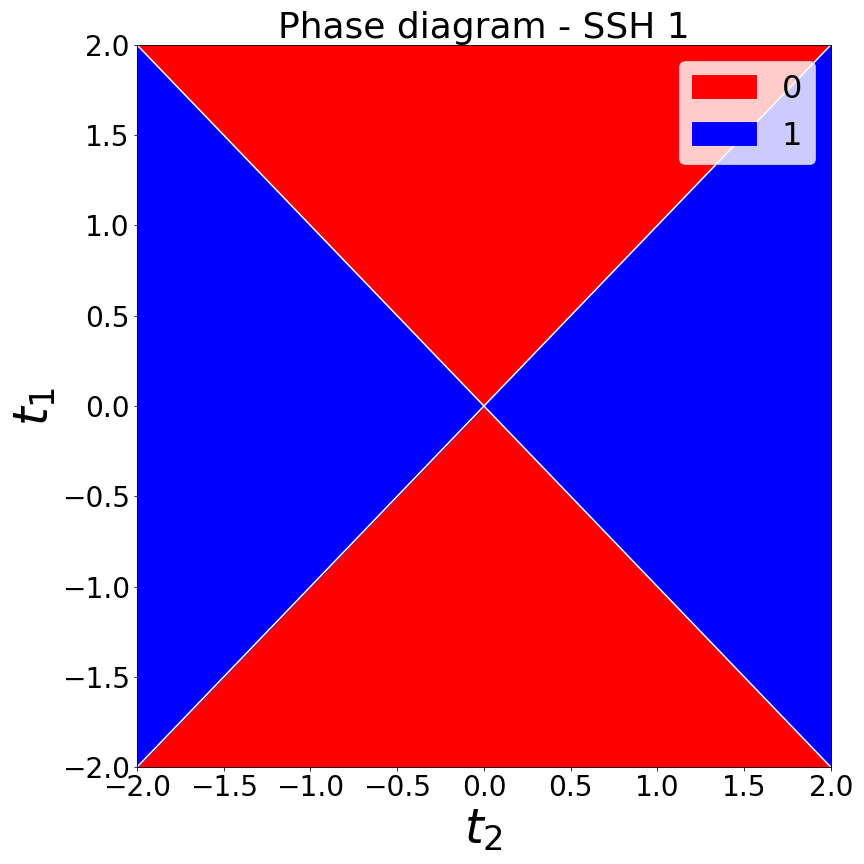
\includegraphics[width=.45\textwidth]{./phase_diagrams/ssh1.png}}\quad
\subfigure[]{\label{ssh2}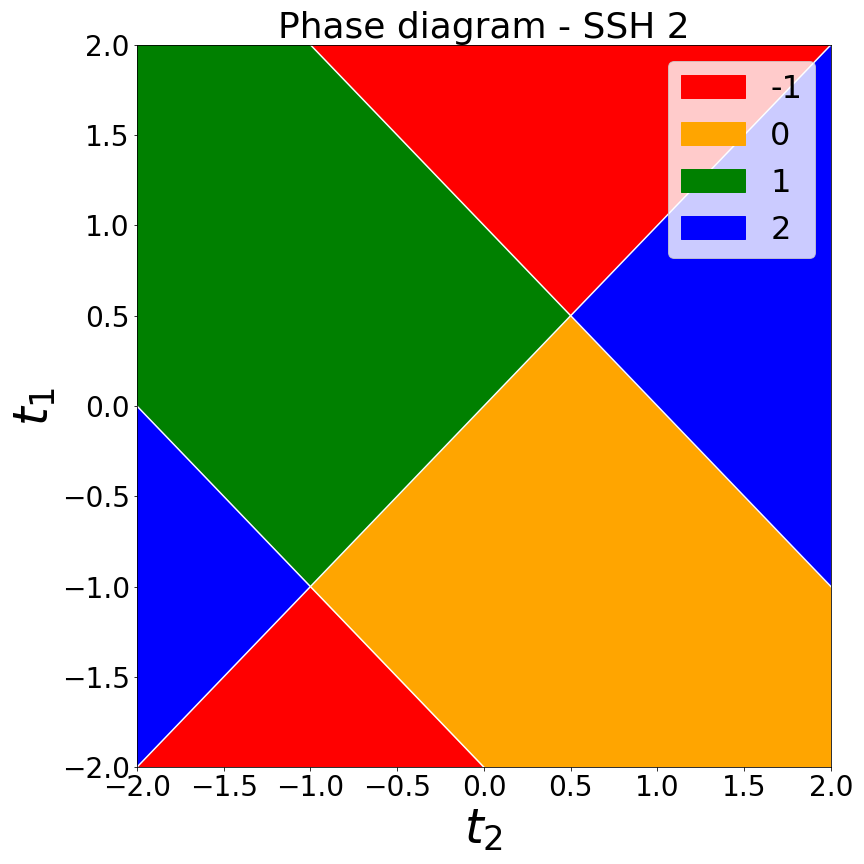
\includegraphics[width=.45\textwidth]{./phase_diagrams/ssh2.png}}
\caption{Phase diagrams in parameter space. a) SSH model with first-neighbor hoppings $t_1$ and $t_2$. The (red) regions with winding number $W$ = 0 are trivial, while the (blue) regions with winding number $W$ = 1 are topologically non-trivial. b) SSH model with first ($t_1$ and $t_2$) and second ($T_1$ and $T_2$) nearest-neighbor hoppings. In this article we set $t_1$ = $t_2$ = 1 and renamed the variables $T_1$ $\rightarrow$ $t_1$, $T_2$ $\rightarrow$ $t_2$ for convenience. The (orange) region with winding number $W$ = 0 is trivial while the others with winding numbers $W$ = -1, $W$ = 1 and $W$ = 2 (red, green and blue respectively) are topologically non-trivial.}
\label{fig:phasediagrams}
\end{figure}

\section{The eigenvector ensembling algorithm}\citequote{eigenvector_ensembling_alg}
\label{the_eigenvector_ensembling_algorithm}
\textcolor{blue}{
The eigenvector ensembling algorithm consists of five steps: 1) Generating Hamiltonians in real space and their corresponding winding numbers; 2) Creating training, validation and test sets; 3) Training on real space eigenvectors of Hamiltonians in the training set; 4) Eigenvector ensembling and 5) Bootstrapping. We describe here in detail each of these steps as they were implemented in this work.
\vspace{.3cm}
\begin{enumerate}%[topsep=0pt, partopsep=0pt]
\item[1)] \textbf{Generating Hamiltonians and winding numbers:} we start generating a number of paremeterized Hamiltonians $H(\mathbf{t})$ in real space and their corresponding winding numbers $W(\mathbf{t})$, where $\mathbf{t} = (t_1, t_2,...,t_h)$ is a vector of $h$ hopping parameters (in the simplest case of the SSH model $h$ = 2). These Hamiltonians are $N\times N$ matrices, where $N$ is twice the number of unit cells in the chain.
\item[2)] \textbf{Creating training, validation and test sets:} we split our set of parameterized Hamiltonians and winding numbers into training, validation and test sets, as is usualy done in machine learning. More explicitly, assume our hopping parameters vector $\mathbf{t}$ takes on the values $\mathbf{t}_1, \mathbf{t}_2, ..., \mathbf{t}_n$ corresponding to the Hamiltonian-winding number pairs ($H_1$, $W_1$), ..., ($H_n$, $W_n$). We partition the set \{($H_i$, $W_i$)$\mid$ $i=1,...,n$\} in three disjoint subsets: the training set, the validation set and the test set.
\item[3)] \textbf{Training on eigenvectors in real space:} since each Hamiltonian $H_i$ is represented by an $N\times N$ matrix, each one will provide $N$ eigenvectors $\mathbf{v}_i^{(1)}, \mathbf{v}_i^{(2)},...,\mathbf{v}_i^{(N)}$ to our data set. Our supervised learning algorithm of choice will take as inputs the real space eigenvectors $\mathbf{v}^{(j)}_i$ of each Hamiltonian $H_i$ in the training set and be trained to learn the winding number $W_i$ of their parent Hamiltonian $H_i$. Therefore, our dataset will consist of eigenvector-winding number pairs $(\mathbf{v}_i^{(j)}, W_i)$.
\item[4)]\textbf{Eigenvector ensembling:} in order to predict the phase of a system described by a particular Hamiltonian we need to take into account how each of its eigenvectors were classified. This amounts to performing ensemble learning on the eigenvectors of each Hamiltonian. In this work we estimate the phase probabilities for each Hamiltonian as the fraction of its eigenvectors that were classified in each phase.
\item[5)] \textbf{Bootstrapping:} We refine the phase probabilities for each Hamiltonian using a bootstrapping procedure, i.e., we repeat steps (1)-(4) $n_\text{exp}$ times, at each round sampling randomly a new training set from our grid in \textbf{t}-space. The final estimated probabilities are then arrived at by averaging the probabilities obtained in each experiment.
\end{enumerate}} 

\vspace{.3cm}
\textcolor{blue}{Before continuing to the analyses of the SSH systems with the eigenvector ensembling algorithm, it will be timely to digress a moment and peek into the algorithm itself. The focus on eigenvectors (and hence the algorithm's name) as the input data to a machine learning algorithm of choice is a hallmark of the procedure as it differentiates it from related applications of machine learning to the study of phase transitions. The intuition that eigenvectors can be used in replacement to raw Hamiltonians can be grasped when we consider the spectral decomposition of a Hamiltonian $H$, }   
\begin{equation}
\label{eigen_decomposition}
H = \sum_{i=1}^{N}\lambda^{(i)} \ket{\mathbf{v}^{(i)}}\bra{\mathbf{v}^{(i)}}
\end{equation}
where $\lambda^{(i)}$ \textcolor{blue}{is the eigenenergy corresponding to the eigenstate $\ket{\mathbf{v}^{(i)}}$. It is therefore clear that all information available from a Hamiltonian can be recovered from its spectral decomposition. By expressing the eigenvectors in a basis suitable to a particular problem (e.g. the real space basis chosen in this article), it becomes possible to investigate the properties of a set of Hamiltonians using the coordinates of eigenvectors in the chosen basis as features. Thus the eigenvector ensembling procedure described above provides a broad framework for the implementation of model explainability in applications to data-driven physics.} 

%\textcolor{blue}{In step 3) we used the implementations of decision trees and random forests from Python's scikit-learn module}\citequote{eigenvector_ensembling_alg}

\section{Numerical experiments}
\label{numerical_experiments}
We performed two numerical experiments with the eigenvector ensembling algorithm. The first experiment deals with the simplest case, the SSH model with nearest-neighbor hopping (here called SSH 1, figure \ref{ssh1}), while the second experiment uses the SSH model with first and second nearest-neighbor hoppings (here called SSH 2, figure \ref{ssh2}).

In each experiment our grid consisted of \nHam\ Hamiltonians uniformly distributed in the closed square $[-2,2]\times[-2,2]$ in the $t_1$-$t_2$ plane in parameter space. The goal in each experiment is to recover the corresponding phase diagram in 2D (two-dimensional) parameter space, figures \ref{ssh1} and \ref{ssh2}, from local lattice data in the much higher-dimensional real space (100D - in both experiments lattices have 50 unit cells, yielding 100$\times$100 Hamiltonian matrices).

This task is particularly hard near phase transition boundaries, where numerical computation of winding numbers become less stable. For this reason, when sampling the training set we only consider those Hamiltonians in the grid whose numerically computed winding numbers lie in a range $\epsilon = \epsilonValue$ around the correct winding number values. Therefore, a good performance metric is the accuracy measured at those Hamiltonians near phase transitions that are never used for training, and thus we assign them to the test set. The remaining Hamiltonians in the grid are split into training and validation sets as detailed in the subsections below.

\textcolor{blue}{As performance metrics, we report here both accuracy of predicted classes for eigenvectors as well as accuracy of predicted classes for Hamiltonians obtained from eigenvector ensembling. These accuracy scores are to be gauged against the baseline of a system that simply guesses the most frequent class for all Hamiltonians. Checking against this baseline is important because it indicates whether the decision trees are in fact learning the underlying patterns that relate real space coordinates to winding numbers, and therefore whether the associated information entropy signature is meaningful or not.}\citequote{sufficient_accuracy} \citequote{evaluation_metrics}

When generating the Hamiltonians we applied periodic boundary conditions to eliminate border effects. This should make recovering a topological signal from local eigenvector coordinates even harder, since in this case the translational symmetry of the systems should allow for no obvious way to distinguish between unit cells. The choice of periodic boundary conditions also implies that the information recovered from real space data comes from the bulk of the topological systems considered and therefore provides strong evidence for the existence of topological signatures in the bulk of such systems. 

Figures \ref{figexp1_exp} and \ref{figexp2_exp} respectively illustrate single iterations of experiment 1 (section \ref{experiment_1}) and experiment 2 (section \ref{experiment_2}) as seen from parameter space. The accuracy statistics presented in the following subsections, as well as the probability heatmaps and recovered phase diagrams shown in figures \ref{ssh1_heatmaps} and \ref{ssh2_heatmaps} were obtained after bootstrapping each experiment $n_{exp}$ = \nExp\ times. \textcolor{blue}{Thus, each probability heatmap shown in figures \ref{ssh1_heatmap_0}-\ref{ssh1_heatmap_1} and \ref{ssh2_heatmap_-1}-\ref{ssh2_heatmap_2} represents the averaged fraction of eigenvectors of each Hamiltonian in the grid that were classified with a given winding number accross $n_{exp}$ experiments. The recovered phase diagrams \ref{ssh1_heatmap} and \ref{ssh2_heatmap} are constructed by superposing the correponding probability heatmaps}. As these figure make clear, the recovered phase diagrams faithfully portray the true phase diagrams in figure \ref{fig:phasediagrams}, with clear phase transition lines appearing in the regions of highest uncertainty.

\textbf{blue}{The numerical experiments with the eigenvector ensembling algorithm described in the next subsections were implemented in Python using the scikit-learn module \cite{scikit}.} 

\subsection{Experiment 1: Learning a first-neighbor hopping SSH model with decision trees}
\label{experiment_1}
Our test set in this experiment contained \sshOneTestNHam\ Hamiltonians (approx. \fpeval{round(\sshOneTestNHam/\nHam*100,\nPrec)}\% of all data). Of the remaining \fpeval{\sshOneTrainNHam+\sshOneValNHam} Hamiltonians, \sshOneTrainNHam\ were randomly assigned to the training set (approx. \fpeval{round(\sshOneTrainNHam/\nHam*100,\nPrec)}\%) and \sshOneValNHam\ (approx. \fpeval{round(\sshOneValNHam/\nHam*100,\nPrec)}\%) were used to compute validation scores at each iteration. These proportions between training and validation sets are such that approximately 10\%  of Hamiltonians from outside of the test set were used for training at each iteration. The composition of the train + validation set for this experiment was \fpeval{round(\sshOneTrainValWindZeroNHam/(\sshOneTrainNHam+\sshOneValNHam)*100,\nPrec)}\% of Hamiltonians with winding number $W$ = 0 and \fpeval{round(\sshOneTrainValWindOneNHam/(\sshOneTrainNHam+\sshOneValNHam)*100,\nPrec)}\% with winding number $W$ = 1. The composition of the test set was \fpeval{round(\sshOneTestWindZeroNHam/(\sshOneTestWindZeroNHam+\sshOneTestWindOneNHam)*100,\nPrec)}\% of Hamiltonians with winding number $W$ = 0 and \fpeval{round(\sshOneTestWindOneNHam/(\sshOneTestWindZeroNHam+\sshOneTestWindOneNHam)*100,\nPrec)}\% with winding number $W=1$. \textcolor{blue}{Our learning algorithm of choice for this experiment was a simple decision tree model \cite{breiman2017classification}}.\citequote{eigenvector_ensembling_alg}

The bootstrap allows us to collect several statistics to evaluate performance. In particular, we report mean accuracies on training eigenvectors (\fpeval{round(\sshOneEigenTrainAcc,\accPrec)}), validation eigenvectors (\fpeval{round(\sshOneEigenValAcc,\accPrec)}) and test eigenvectors (\fpeval{round(\sshOneEigenTestAcc,\accPrec)}). Eigenvector ensembling substantially improved mean accuracies for Hamiltonians. These were \fpeval{round(\sshOneHamTrainAcc,\accPrec)} for training Hamiltonians, \fpeval{round(\sshOneHamValAcc,\accPrec)} for validation Hamiltonians and \fpeval{round(\sshOneHamTestAcc,\accPrec)}  for test Hamiltonians. \textcolor{blue}{When compared with the baseline test accuracy of \fpeval{round(\sshOneTestWindOneNHam/(\sshOneTestWindZeroNHam+\sshOneTestWindOneNHam),\accPrec)} of a system that predicts the whole test set as having winding number $W=1$, the accuracy of \fpeval{round(\sshOneHamTestAcc,\accPrec)} on test Hamiltonians indicates that the decision trees indeed learned the patterns that relate real space coordinates to winding numbers.} \citequote{sufficient_accuracy}

The probability heatmaps and phase diagram learned by the combination of decision trees with eigenvector ensembling used in experiment 1 are shown in figure \ref{ssh1_heatmaps}. 

\begin{figure}
\centering
\subfigure[]{\label{figexp1_exp:a}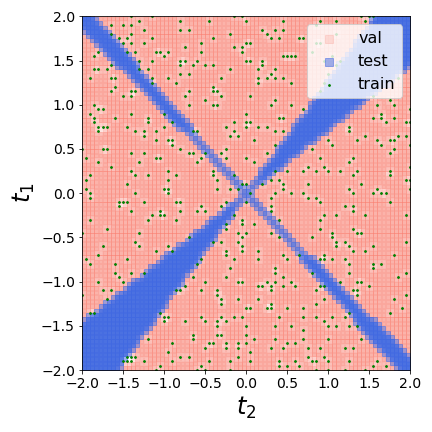
\includegraphics[width=.32\textwidth]{./ssh1/periodic_100_6561/scatter_train_val_test_experiment_0.png}}\quad
\subfigure[]{\label{figexp1_exp:b}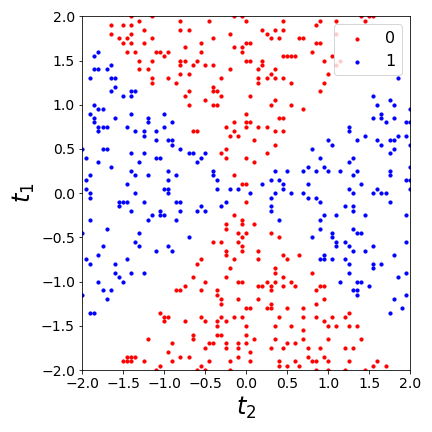
\includegraphics[width=.32\textwidth]{./ssh1/periodic_100_6561/scatter_winding_train_experiment_0.png}}
\subfigure[]{\label{figexp1_exp:c}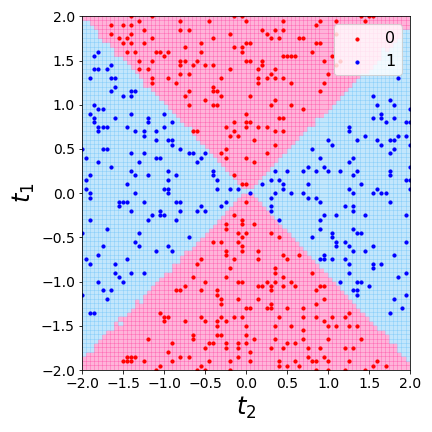
\includegraphics[width=.32\textwidth]{./ssh1/periodic_100_6561/pcolormesh_prediction_grid_experiment_0.png}}
\caption{Visualization of a single iteration of experiment 1 (section \ref{experiment_1}) as seen from 2D parameter space. (a) Train/validation/test split. (b) Distribution of winding numbers in the training set. (c) Phase diagram learned from real space lattice data by a combination of decision tree and eigenvector ensembling.}
\label{figexp1_exp}
\end{figure}

\subsection{Experiment 2: Learning a first- and second-neighbor hoppings SSH model with random forests}
\label{experiment_2}

This task is considerably more difficult than the previous one due to the higher number of classes and the fact that some of the labels encompass disconnected regions. For this reason, instead of using a single decision tree, we upgraded our model to a random forest \cite{Breiman2001} with \nEst\ decision trees. Our data set consisted of \sshTwoTestNHam\ (\fpeval{round(\sshTwoTestNHam/\nHam*100,\nPrec)}\%) test Hamiltonians. The remaining Hamiltonians are randomly split in half between training and validation sets at each iteration, giving \sshTwoTrainNHam\ (\fpeval{round(\sshTwoTrainNHam/\nHam*100,\nPrec)}\%) training Hamiltonians and \sshTwoValNHam\ (\fpeval{round(\sshTwoValNHam/\nHam*100,\nPrec)}\%) validation Hamiltonians. The distribution of winding numbers for the Hamiltonians in the train + validation set for this experiment was $W$ = -1 (\fpeval{round(\sshTwoTrainValWindMinusOneNHam/(\sshTwoTrainNHam+\sshTwoValNHam)*100,\nPrec)}\%), $W$ = 0 (\fpeval{round(\sshTwoTrainValWindZeroNHam/(\sshTwoTrainNHam+\sshTwoValNHam)*100,\nPrec)}\%), $W$ = 1 (\fpeval{round(\sshTwoTrainValWindOneNHam/(\sshTwoTrainNHam+\sshTwoValNHam)*100,\nPrec)}\%) and $W$ = 2 (\fpeval{round(\sshTwoTrainValWindTwoNHam/(\sshTwoTrainNHam+\sshTwoValNHam)*100,\nPrec)}\%). The distribution of winding numbers for the Hamiltonians in the test set was $W$ = -1 (\fpeval{round(\sshTwoTestWindMinusOneNHam/(\sshTwoTestWindMinusOneNHam+\sshTwoTestWindZeroNHam+\sshTwoTestWindOneNHam+\sshTwoTestWindTwoNHam)*100,\nPrec)}\%), $W$ = 0 (\fpeval{round(\sshTwoTestWindZeroNHam/(\sshTwoTestWindMinusOneNHam+\sshTwoTestWindZeroNHam+\sshTwoTestWindOneNHam+\sshTwoTestWindTwoNHam)*100,\nPrec)}\%), $W$ = 1 (\fpeval{round(\sshTwoTestWindOneNHam/(\sshTwoTestWindMinusOneNHam+\sshTwoTestWindZeroNHam+\sshTwoTestWindOneNHam+\sshTwoTestWindTwoNHam)*100,\nPrec)}\%) and $W$ = 2 (\fpeval{round(\sshTwoTestWindTwoNHam/(\sshTwoTestWindMinusOneNHam+\sshTwoTestWindZeroNHam+\sshTwoTestWindOneNHam+\sshTwoTestWindTwoNHam)*100,\nPrec)}\%).

Mean accuracies across \nExp\ repetitions of experiment 2 were \fpeval{round(\sshTwoEigenTrainAcc,\accPrec)} for training eigenvectors, \fpeval{round(\sshTwoEigenValAcc,\accPrec)} for validation eigenvectors and \fpeval{round(\sshTwoEigenTestAcc,\accPrec)} for test eigenvectors. Mean accuracies resulting from eigenvector ensembling were \fpeval{round(\sshTwoHamTrainAcc,\accPrec)} for training Hamiltonians, \fpeval{round(\sshTwoHamValAcc,\accPrec)} for validation Hamiltonians and \fpeval{round(\sshTwoHamTestAcc,\accPrec)} for test Hamiltonians. The large accuracy gain achieved by eigenvector ensembling in the test set (going from \fpeval{round(\sshTwoEigenTestAcc,\accPrec)} eigenvector accuracy to \fpeval{round(\sshTwoHamTestAcc,\accPrec)} Hamiltonian accuracy) attests to its power. The effectiveness of eigenvector ensembling is also evident from the much worse performance (\fpeval{round(\sshTwoTestWindTwoNHam/(\sshTwoTestWindMinusOneNHam+\sshTwoTestWindZeroNHam+\sshTwoTestWindOneNHam+\sshTwoTestWindTwoNHam),\accPrec)}) achieved by a baseline system that simply guesses $W=2$ for all test Hamiltonians in this experiment. 



The probability heatmaps and phase diagram learned by the combination of random forests with eigenvector ensembling used in experiment 2 are shown in figure \ref{ssh2_heatmaps}.

\begin{figure}
\centering
\subfigure[]{\label{figexp2_exp:a}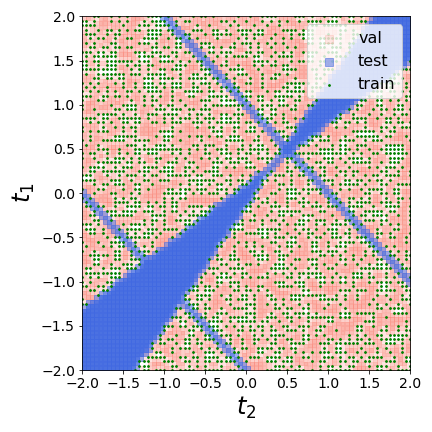
\includegraphics[width=.32\textwidth]{./ssh2/periodic_100_6561/scatter_train_val_test_experiment_0.png}}\quad
\subfigure[]{\label{figexp2_exp:b}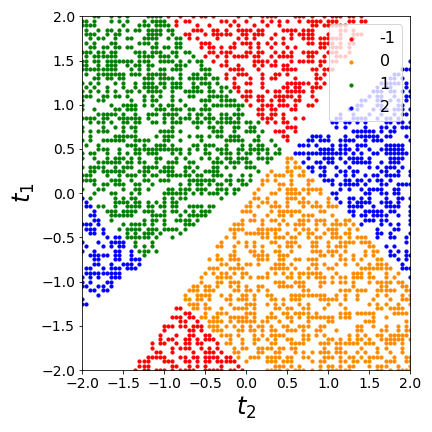
\includegraphics[width=.32\textwidth]{./ssh2/periodic_100_6561/scatter_winding_train_experiment_0.png}}
\subfigure[]{\label{figexp2_exp:c}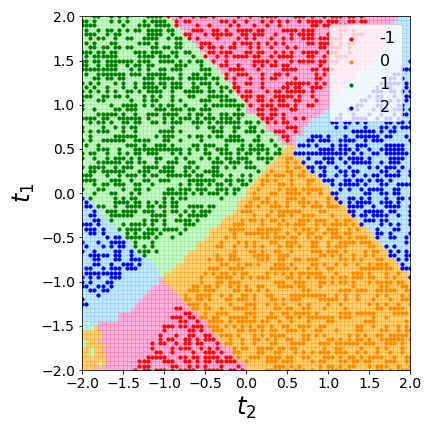
\includegraphics[width=.32\textwidth]{./ssh2/periodic_100_6561/pcolormesh_prediction_grid_experiment_0.png}}
\caption{Visualization of a single iteration of experiment 2 (section \ref{experiment_2}) as seen from 2D parameter space. (a) Train/validation/test split. (b) Distribution of winding numbers in the training set. (c) Phase diagram learned from real space lattice data by a combination of random forest and eigenvector ensembling.}
\label{figexp2_exp}
\end{figure}

\section{Information entropy signatures}
\label{information_entropy_signatures}

We now analyze how the algorithm was able to recover a global property of the Hamiltonians (their topological phase) from bulk local features (real space eigenvector coordinates on each lattice site). Alongside the fact that decision trees and random forests are very easy to train and visualize, the other reason that led us to test our algorithm with them was that they allow us to check which features (and thus which lattice sites) were most informative in training.

The (normalized) relevance of a feature is given by how much it reduces a loss function (e.g. Shannon information entropy or Gini impurity \cite{friedman2001elements}). By averaging normalized relevances as measured by reduction in the information entropy of ensembles of real space eigenvectors across $n_{exp}$ = 100 iterations of both experiment 1 (section \ref{experiment_1}) and experiment 2 (section \ref{experiment_2}) we recovered Shannon entropy signals that reveal which lattice sites were consistently more relevant in learning topological phases from data in real space for each experiment. These signals are the information entropy signatures of each topological phase transition. 

The bar plots in figure \ref{feature_importances} show how informative each lattice site was in learning topological phases for each experiment. They represent the information entropy signatures along the lattices in each SSH system. For experiment 1 (section \ref{experiment_1}), only six lattice sites (0, 1, 3, 50, 51, 53) corresponding to the two sharp peaks seen in figure \ref{feature_importances_ssh1} contributed approximately 70\% of total reduction in Shannon entropy. Similarly, approximately 30\% of total reduction in the Shannon information entropy of eigenvector data from experiment 2 (section \ref{experiment_2}) was achieved by eighteen lattice sites(0, 1, 2, 3, 4, 5, 46, 48, 49, 50, 51, 53, 94, 95, 96, 97, 98, 99) distributed along the three peaks in figure \ref{feature_importances_ssh2}. As we shall see in section \ref{topological_feature_engineering}, the information entropy signatures can be used to compress the topological information in SSH lattices.

\textcolor{blue}{We should remark on the subtleties of the information entropy signatures presented here. Although they give us a visualization of how important each lattice site was in determining the topological phases of Hamiltonians, they actually express a global property of the whole lattice. In the next section, where we develop a quantum formalism for the information entropy signatures discovered in this section, these seemingly antagonistic conceptions shall be harmonized. What is important to emphasize at this point is that the information entropy signature should not be naively taken at face value: a lattice site that appears unimportant in an information entropy signature plot may not be unimportant or void of topological information by itself.}

\textcolor{blue}{To give a concrete example, reduction in Shannon entropy tends to be distributed among highly correlated variables. This implies that if only a single lattice site in a highly correlated subset is used by a learning algorithm, it will likely inherit most of the reduction in Shannon entropy from the other correlated lattice sites that were not taken into account by the algorithm. The corollary of this fact is that lattice sites that carry redundant information that is also available from other lattice sites tend to have decreased importance in the information entropy signature.  In this regard the information entropy signatures presented here express a summary of relations between lattice sites and are therefore intrinsically global.} 

%Another important point to be emphasized is that these signals were recovered from the analysis of data from several thousand SSH systems in %each experiment and therefore they are not a property of a single SSH lattice. They are rather a pattern that emerges from correlating %topological winding numbers with lattice eigenvector data for several SSH systems.   

\textcolor{blue}{Each of the information entropy signatures shown in figure \ref{feature_importances} captures a general pattern that persists regardless of the length of the lattice (i.e., the number of unit cells) used to compute them. In fact, by rerunning each experiment with longer lattices we have verified that the signals in figures \ref{feature_importances_ssh1} and \ref{feature_importances_ssh2} appear to converge to well defined continuous density functions in the macroscopic limit. They are not, therefore, artifacts of particular choices of hyperparameters used to run the eigenvector ensembling algorithm. The information entropy signatures for longer lattices are presented in the section \textbf{Numerical explorations on longer lattices} in the Supplementary Material.}

%The macroscopic limit of these information entropy signals may be an important signature of topological systems and thus merits further %theoretical investigation. This is pursued in the next section. We present the information entropy signatures for longer lattices in the %section \textbf{Numerical explorations on longer lattices} in the Supplementary Material.}

%To see if learning the topological phases can be achieved efficiently by employing simpler models we reran each experiment using only a small %subset of most relevant lattice sites. In our rerun of experiment 1 (section \ref{experiment_1}) using only lattice sites $S'_1$ = (0, 50, %51, 99) (which contributed approximately 45 \% of total reduction in Shannon information entropy), mean accuracies were 97.0\% for training %eigenvectors, 91.5\% for validation eigenvectors and 72.8\% for test eigenvectors. Mean accuracies obtained from eigenvector ensembling were %99.1\% for training Hamiltonians, 99.5\% for validation Hamiltonians and 94.5\% for test Hamiltonians.

%Mean accuracies for our rerun of experiment 2 (section \ref{experiment_2}) using only lattice sites $S'_2$ = (0, 1, 3, 48, 50, 51, 96, 98, %99) (which contributed approximately 20 \% of total reduction in Shannon information entropy) were 99.9\% for training eigenvectors, 87.7\% %for validation eigenvectors and 47.3\% for test eigenvectors. Eigenvector ensembling yields mean accuracies of 100\% for training %Hamiltonians, 99.5\% for validation Hamiltonians and 74.5\% for test Hamiltonians.  


\begin{figure}
\centering
\subfigure[]{\label{ssh1_heatmap_0}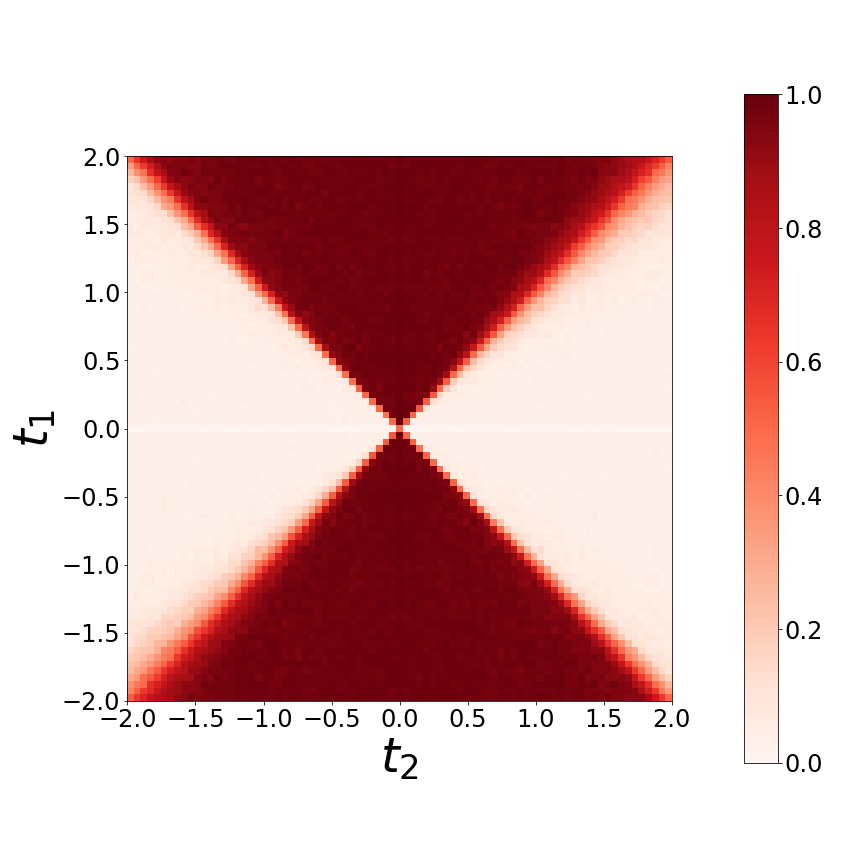
\includegraphics[width=.32\textwidth]{./ssh1/periodic_100_6561/imshow_winding_grid_winding_0_sim.png}}
\subfigure[]{\label{ssh1_heatmap_1}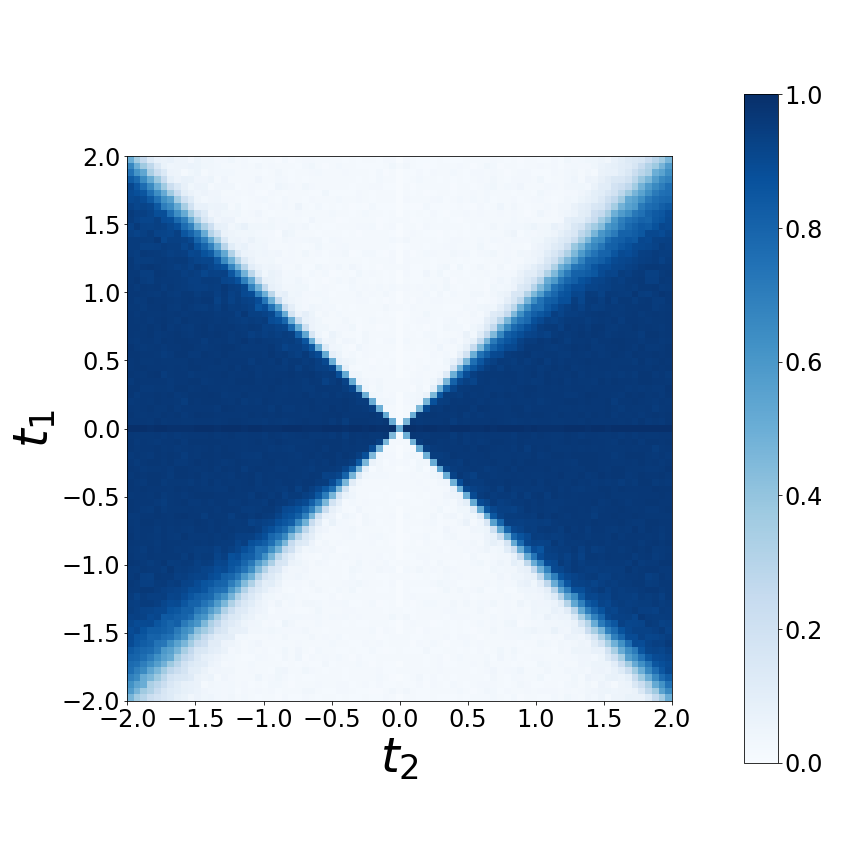
\includegraphics[width=.32\textwidth]{./ssh1/periodic_100_6561/imshow_winding_grid_winding_1_sim.png}}
\subfigure[]{\label{ssh1_heatmap}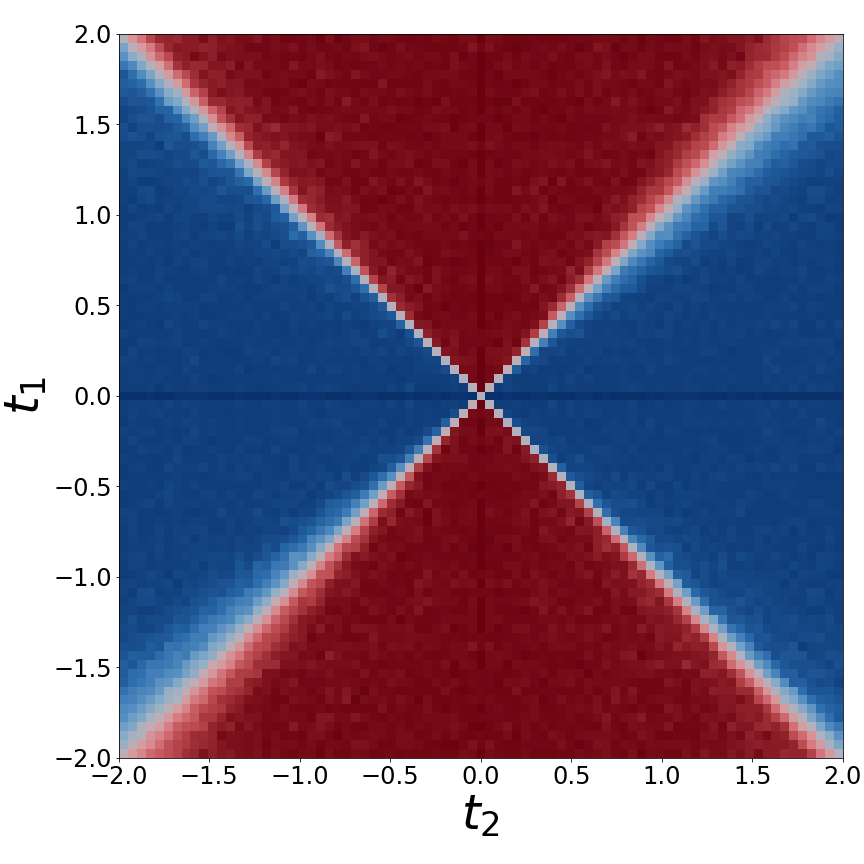
\includegraphics[width=.32\textwidth]{./ssh1/periodic_100_6561/merge_imshow_winding_grids_second_sim.png}}
\caption{Probability heatmaps learned by a combination of decision trees with eigenvector ensembling from bulk real space eigenvector data in experiment 1 (section \ref{experiment_1}). Heatmaps were averaged across all 100 iterations of the experiment. (a) Probability heatmap showing the probability that a Hamiltonian in the grid has winding number equal to 0.  (b) Probability heatmap showing the probability that a Hamiltonian in the grid has winding number equal to 1. (c) The phase diagram resulting from heatmaps (a) and (b).}
\label{ssh1_heatmaps}
\end{figure}

\begin{figure}
\centering
\subfigure[]{\label{ssh2_heatmap_-1}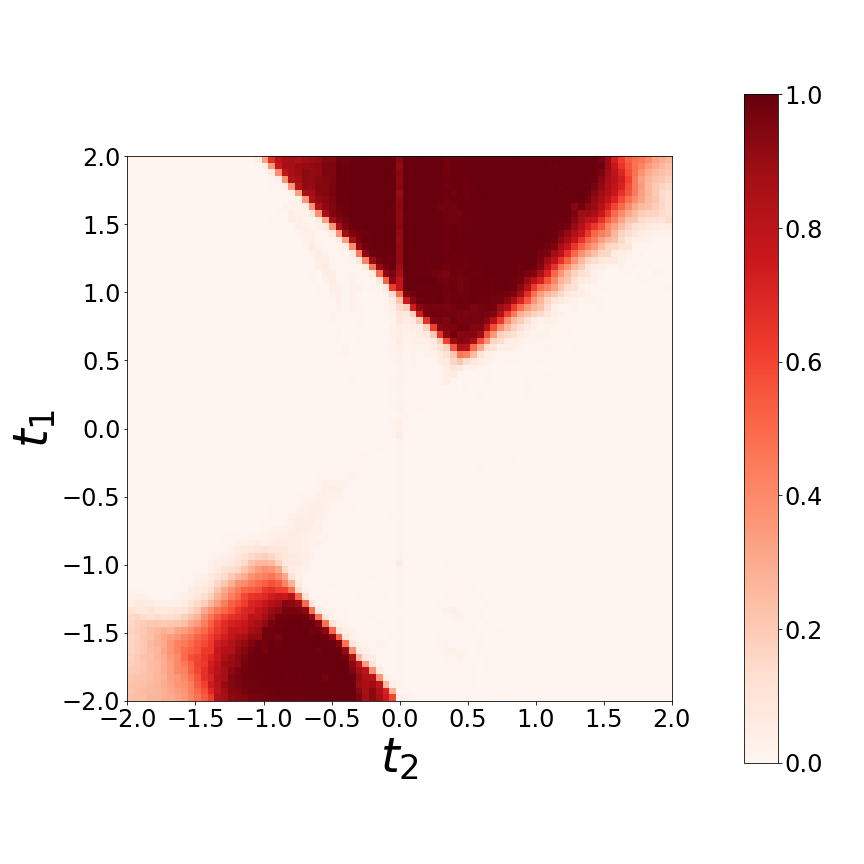
\includegraphics[width=.32\textwidth]{./ssh2/periodic_100_6561/imshow_winding_grid_winding_-1_sim.png}}
\subfigure[]{\label{ssh2_heatmap_0}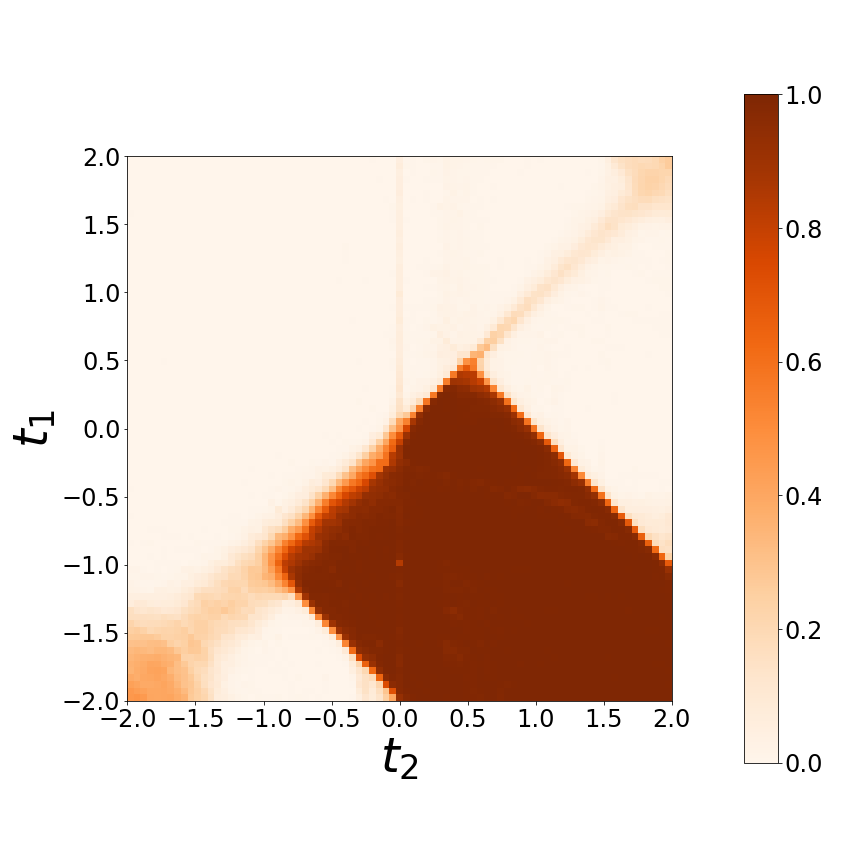
\includegraphics[width=.32\textwidth]{./ssh2/periodic_100_6561/imshow_winding_grid_winding_0_sim.png}}
\subfigure[]{\label{ssh2_heatmap_1}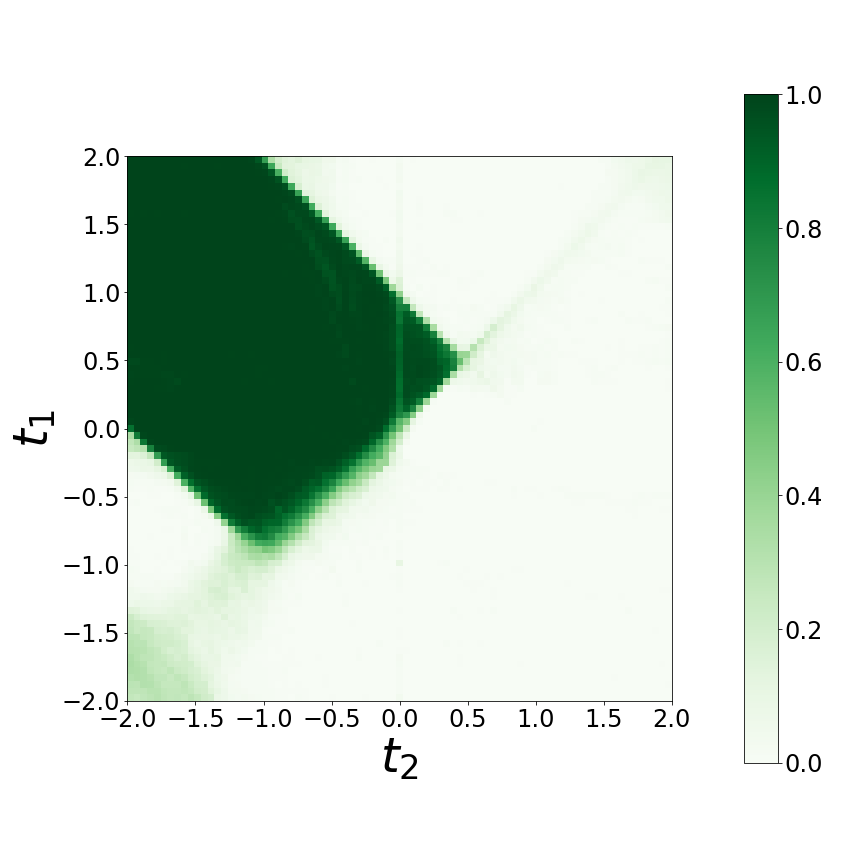
\includegraphics[width=.32\textwidth]{./ssh2/periodic_100_6561/imshow_winding_grid_winding_1_sim.png}}
\subfigure[]{\label{ssh2_heatmap_2}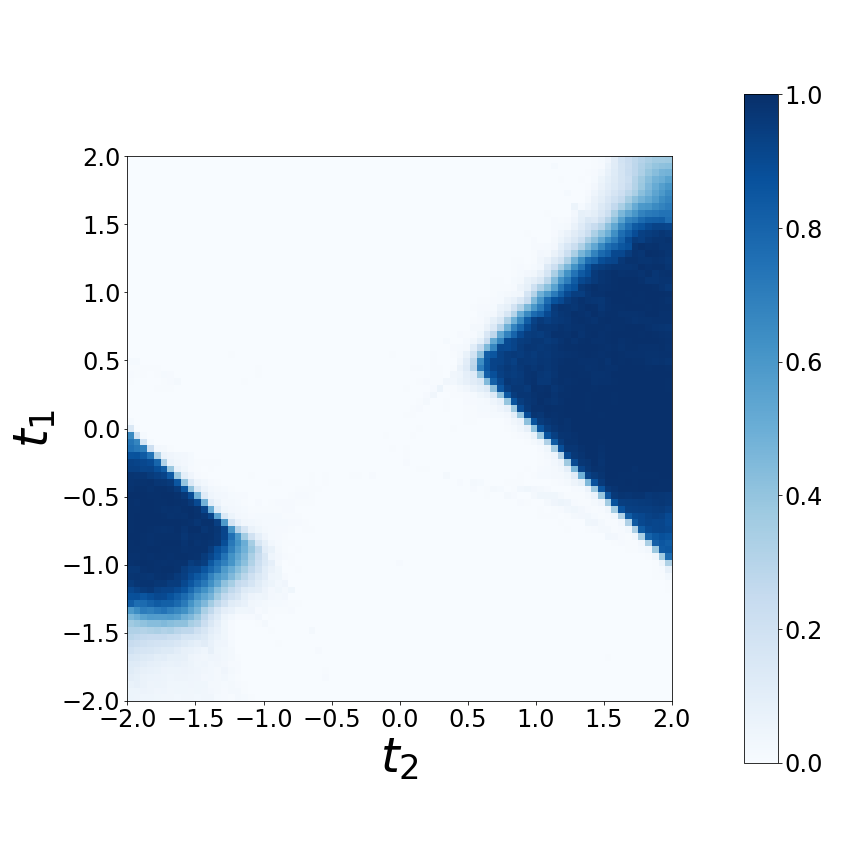
\includegraphics[width=.32\textwidth]{./ssh2/periodic_100_6561/imshow_winding_grid_winding_2_sim.png}}
\subfigure[]{\label{ssh2_heatmap}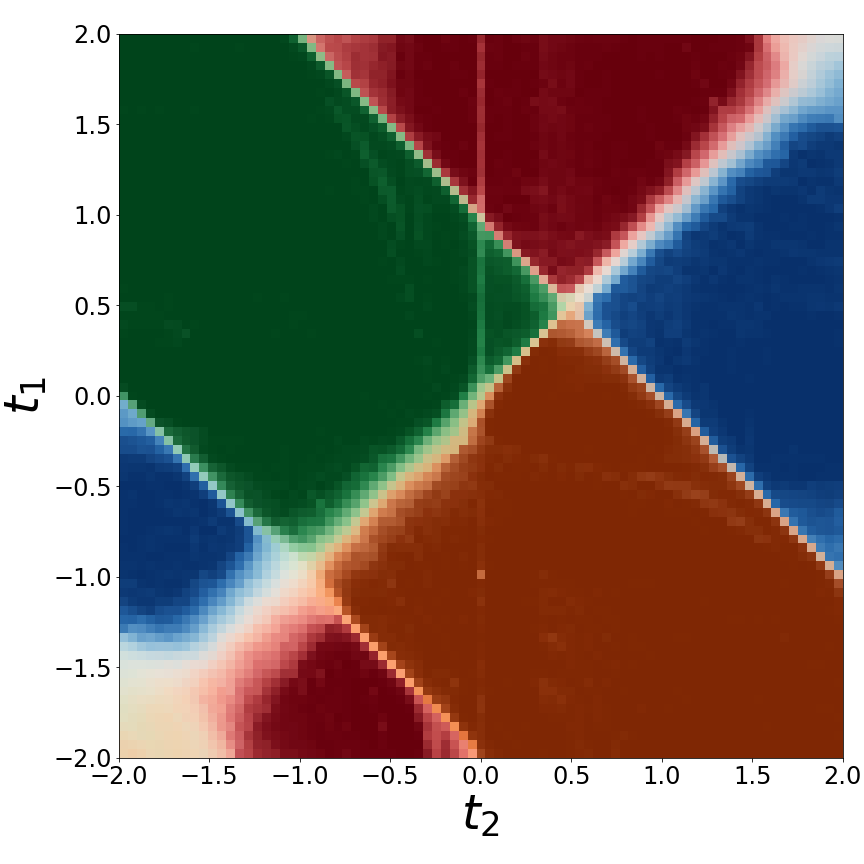
\includegraphics[width=.32\textwidth]{./ssh2/periodic_100_6561/merge_imshow_winding_grids_sim.png}}
\caption{Probability heatmaps learned by a combination of random forests with eigenvector ensembling from bulk real space eigenvector data in experiment 2 (section \ref{experiment_2}). Heatmaps were averaged across all 100 iterations of the experiment. (a) Probability heatmap showing the probability that a Hamiltonian in the grid has winding number equal to -1.  (b) Probability heatmap showing the probability that a Hamiltonian in the grid has winding number equal to 0. (c) Probability heatmap showing the probability that a Hamiltonian in the grid has winding number equal to 1. (d) Probability heatmap showing the probability that a Hamiltonian in the grid has winding number equal to 2. (e) The phase diagram resulting from heatmaps (a)-(d).}
\label{ssh2_heatmaps}
\end{figure}


\section{Topological feature engineering and lattice compression}
\label{topological_feature_engineering}

In this section, we explore the information entropy signatures obtained in section \ref{information_entropy_signatures} from an information-theoretic perspective, in particular as related to data compression. As we have argued at the end of section \ref{information_entropy_signatures}, the information entropy signatures can be used as a powerful dimensionality reduction tool: by keeping only the most relevant lattice sites in an information entropy signature, the amount of data needed to characterize the topological phase of a SSH system can be largely decreased with little loss of information. Nevertheless, given that the topological phase of a SSH system is a global property of the whole lattice, it is natural to expect that it should be possible to engineer global features from real space coordinates. Here we show how the symmetries in the real space information entropy signatures in figure \ref{feature_importances} can be exploited to engineer new global topological features, leading to an effective compression of topological information.

%simply extracting local coordinates of real space eigenvectors may not be the most effective way to condense a lattice's topological %information. Here we explore the engineering of new global topological features in real space, and how these global features lead to an %effective compression of topological information. 

%The information entropy signatures in wavevector space can be easily computed from their counterparts in real space (figures %\ref{feature_importances_ssh1} and \ref{feature_importances_ssh2}) using equation \eqref{fourier_shannon_wave_function} and assuming that the %real space information entropy wave functions are real. 

Given a real space eigenvector $x[m]$, we can compute its coordinates in wavevector space using the Discrete Fourier Transform (DFT),  
\begin{equation}
\label{discrete_fourier_transform}
\hat{x}[n] = \frac{1}{\sqrt{N}}\sum_{m=0}^{N-1}x[m]e^{-i\frac{2\pi}{N}nm}, \quad n=0,\dots,N-1.
\end{equation}
Since the choice of phase of the real space eigenvectors was such that they were all in $\mathbb{R}^{N}$, the eigenvectors in wavevector space computed from equation \eqref{discrete_fourier_transform} will be Hermitian vectors in $\mathbb{C}^N$. The Hermitian symmetry of the wavevector space eigenvectors manifests itself mathematically in closed lattices with periodic boundary conditions as 
\begin{equation}
\label{hermitian_symmetry}
\hat{x}[\overline{k}] = \hat{x}^*[\overline{N-k}], \quad k = 0,\dots, N-1,
\end{equation}
where  we have used the notation $\overline{k} = k \mod N$. 

Equation \eqref{hermitian_symmetry} forks into two natural paths to topological feature engineering. In the first path, we exploit the fact that the real part of $\hat{x}[m]$ is even-symmetric around the reciprocal lattice sites $0$ and $\frac{N}{2}$. This leads us to the Discrete Cosine Transform (DCT) topological features,
\begin{equation}
\label{DCT}
\hat{x}^{c}[n] = x[0] + (-1)^n x[M-1] + \sum_{m=1}^{M-2} 2x[m]\cos\bigg(\frac{\pi}{M-1}nm\bigg), \quad n=0,\dots,M-1, 
\end{equation}
where $M = \frac{N}{2}+1$. The second path capitalizes on the fact that de imaginary part of $\hat{x}[m]$ is odd-symetric around the reciprocal lattice sites $0$ and $\frac{N}{2}$, thus yielding the Discrete Sine Transform (DST) topological features,
\begin{equation}
\label{DST}
\hat{x}^{s}[n] = \sum_{m=0}^{M-1} 2x[m+1]\sin\bigg(\frac{\pi}{M+1}(n+1)(m+1)\bigg), \quad n=0,\dots,M-1,
\end{equation} 
where $M = \frac{N}{2}-1$. 

The topological features in both equations \eqref{DCT} and \eqref{DST} are generated from only half of the real space lattice, i.e. the sites $0 \leq j \leq \frac{N}{2}$. This is due to the fact that each equation assumes that the real space eigenvectors are even-symmetric (DCT topological features) or odd-symmetric (DST topological features) around the lattice sites $0$ and $\frac{N}{2}$ in real space as well. While these assumptions are strictly true for the eigenvector representations in wavevector space, this is not generally true for the real space representations. Therefore, equations \eqref{DCT} and \eqref{DST} achieve lattice compression by keeping only half of the real space eigenvector coordinates and imposing the corresponding boundary conditions (even symmetry or odd symmetry) on the lattice sites $0$ and $\frac{N}{2}$ to extrapolate the information from half of the lattice in real space. 

The topological feature engineering strategies described above are commonly employed in several applications of Digital Signal Processing like audio and image processing and, most importantly here, data compression. As equations \eqref{DCT} and \eqref{DST} show, signal transforms such as the DCT and DST profit from the redundance of information arising from certain symmetries in signals, allowing us to write a signal of length $N$ in terms of at most $M = \frac{N}{2}+1$ features. 
   
We ran several numerical experiments to evaluate if the DCT and DST topological features defined in equations \eqref{DCT} and \eqref{DST}  are able to efficiently encode the topological information existing in SSH lattices. The accuracy scores obtained in each experiment are listed in table \ref{numerical_results}, where we also report the accuracy scores of the numerical experiments of section \ref{numerical_experiments}.

The lattice compression strategies tested in this work were: i) learning topological phases from only a subset of the real space lattice sites; ii) learning topological phases from the DCT or DST engineered features of equations; iii) learning topologcal phases from a fraction of the DCT or DST topological features and iv) learning topological phases from a fraction of the DCT or DST features, computed from only a fraction of real space lattice sites. 

In strategy \emph{i)} the lattice sites used in the SSH1 and SSH2 systems were
\begin{equation}
\label{lattice_subsets}
\mathcal{S}_1 = (0, 1, 3, 50 ) \quad \text{and} \quad  \mathcal{S}_2 =(0, 1, 2, 3, 4, 5, 6, 7, 46, 48, 49, 50).   
\end{equation}
Note that for the nearest-neighbor SSH system $\mathcal{S}_1$ correspond to the four most informative sites such that $0\leq j \leq 50$ as indicated by the information entropy signature in figure \ref{feature_importances_ssh1}. Similarly, for the first- and second- nearest neighbors SSH system $\mathcal{S}_2$ correspond to the twelve most informative sites such that $0\leq j \leq 50$ in the corresponding information entropy signature in figure \ref{feature_importances_ssh2}. In table \ref{numerical results}, the features used in strategy \emph{i)} are referred to as $X_{\mathcal{S}_1}$ and $X_{\mathcal{S}_2}$, according to the SSH system they relate to.  

In strategy \emph{ii)}, the full set of DCT or DST topological features written in equations \eqref{DCT} and \eqref{DST} were used. These features are denoted in table \ref{numerical_results} by $\hat{X}^c_1$, $\hat{X}^s_1$, $\hat{X}^c_2$, $\hat{X}^s_2$ according to which set of topological features and SSH systems they refer to. 

Similarly to strategy \emph{i)}, in strategy \emph{iii)} we selected the DCT topological features used in the SSH1 and SSH2 systems,
\begin{equation}
\label{DCT_subsets}
\mathcal{E}_1 = (1, 2, 36, 49) \quad \text{and} \quad  \mathcal{E}_2 =(0, 1, 2, 3, 4, 5, 6, 7, 47, 48, 49, 50) \qquad \text{(DCT)}  
\end{equation}
and the DST topological features,
\begin{equation}
\label{DST_subsets}
\mathcal{O}_1 =  (0, 18, 28, 30) \quad \text{and} \quad  \mathcal{O}_2 = (0, 1, 2, 3, 4, 5, 43, 44, 45, 46, 47, 48) \qquad \text{(DST)}.  
\end{equation}
The features in strategy \emph{iii)} are denoted in table \ref{numerical_results} by $\hat{X}^c_{\mathcal{E}_1}$, $\hat{X}^s_{\mathcal{O}_1}$, $\hat{X}^c_{\mathcal{E}_2}$, $\hat{X}^s_{\mathcal{O}_2}$ according to the topological features and wavevector sites used with each SSH system. 

The most aggressive lattice compression strategy tested in this work was strategy \emph{iv)}. It consists of using the DCT (DST) topological features of equation \eqref{DCT_subsets} (equation \eqref{DST_subsets}), but having computed these topological features using only the real space lattice sites given in equation \eqref{lattice_subsets}. Thus in strategy \emph{iv)} a lossy compression is performed both on real space features and the engineered DCT (DST) topological features. Mathematically, we can expess the topological features used in strategy \emph{iv)} as follows:
\begin{equation}
\label{DCT_very_compressed}
\hat{x}_{\mathcal{S}, \mathcal{E}}^c[n] = \mathbbm{1}_{\mathcal{S}}[0]x[0] + (-1)^n\mathbbm{1}_{\mathcal{S}}[M-1] x[M-1] + \sum_{m \in \mathcal{S}} 2x[m]\cos\bigg(\frac{\pi}{M-1}nm\bigg), \quad n \in \mathcal{E} \qquad \text{(DCT)} 
\end{equation}
\begin{equation}
\label{DST_very_compressed}
\hat{x}_{\mathcal{S}, \mathcal{O}}^s[n] = \sum_{m \in \mathcal{S}}2x[m+1]\sin\bigg(\frac{\pi}{M+1}(n+1)(m+1)\bigg), \quad n \in \mathcal{O} \qquad \text{(DST)}.
\end{equation}
where in equation \eqref{DCT_very_compressed} the notation $\mathbbm{1}_{\mathcal{S}}[j]$ stands for the indicator function of the lattice subset $\mathcal{S}$, i.e. $\mathbbm{1}_{\mathcal{S}}[j] = 1$ if $j \in \mathcal{S}$ and $\mathbbm{1}_{\mathcal{S}}[j] = 0$ otherwise. The features engineered in strategy \emph{iv)} are denoted in table \ref{numerical_results} by $\hat{X}^c_{\mathcal{S}_1,\mathcal{E}_1}$, $\hat{X}^s_{\mathcal{S}_1,\mathcal{O}_1}$, $\hat{X}^c_{\mathcal{S}_2,\mathcal{E}_2}$, $\hat{X}^s_{\mathcal{S}_2,\mathcal{O}_2}$, again referencing the appropriate SSH system, type of topological features used as well as which features in real and wavevector space were used to engineer them. 

The results shown in table \ref{numerical_results} carry some important surprises. For example, the topological phase transition boundaries of SSH-1 systems can be learned using only the four real space lattice sites $\mathcal{S}_1$ with virtually no loss in accuracy, as seen from eigenvector and Hamiltonian accuracy scores in the . The same appears to be true to SSH-2 systems, where the twelve real space lattice sites $\mathcal{S}_2$ produce accuracy scores at near the same level as using the whole lattice.    

Even more striking is the performance achieved by the DCT topological features $\hat{X}^c_{\mathcal{S},\mathcal{E}}$ defined in equation \eqref{DCT_very_compressed}. For SSH-1 systems, they perform on par with using the full set of real space features $X_1$, while for SSH-2 systems a small loss in accuracy is incurred.

Another interesting insight comes from comparing the accuracy scores obtained with DCT topological features versus DST topological features. The latter seems to have poorer performance than the former, as is indicated by the sharp drop in accuracy scores obtained with the DST topological features $\hat{X}^s_{\mathcal{S},\mathcal{O}}$ in both SSH-1 and SSH-2 systems. This may be related to the fact that the odd-symmetric boundary conditions imposed on DST topological features imply discarding the lattice sites 0 and $50$, which correspond to sharp peaks in the information entropy signatures of figures \ref{feature_importances_ssh1} and \ref{feature_importances_ssh2}.  

The accuracy scores obtained with the real space features $X_{\mathcal{S}_\alpha}$ and the DCT topological features $\hat{X}^c_{\mathcal{S}_\alpha,\mathcal{E}_\alpha}$, both of which use information from a small fraction of real space lattice sites, demonstrate that learning topological phases from local real space data in the bulk is still possible even for small subsets of lattice sites. \textcolor{blue}{In this sense, key topological information can be said to be localized on few sites in the lattice.}\citequote{key_top} We refer the reader to the section \textbf{Learning topological phases from real space data} in the Supplementary Material for a discussion of how this is possible.       



\begin{table}
 \begin{tabular}{||c@{\hskip 0.3in} c@{\hskip 0.3in} c@{\hskip 0.3in} c@{\hskip 0.3in} c@{\hskip 0.3in} c||} 
 \hline
SSH systems &Features                              &Val. eigenvectors  &Test eigenvectors  &Val. Hamiltonians          &Test Hamiltonians  \\  
 \hline\hline
            &                                              &               &                    &                      &                   \\
1           &\xOne                                         &\xOneEigVal    &\xOneEigTest        &\xOneHamVal           &\xOneHamTest       \\
\hline
1           &\xSOne                                        &\xSOneEigVal   &\xSOneEigTest       &\xSOneHamVal          &\xSOneHamVal       \\
\hline
1           &\xcOne                                        &\xcOneEigVal   &\xcOneEigTest       &\xcOneHamVal          &\xcOneHamTest      \\
\hline
1           &\xcEOne                                       &\xcEOneEigVal  &\xcEOneEigTest      &\xcEOneHamVal         &\xcEOneHamTest     \\
\hline
1           &\xcSEOne                                      &\xcSEOneEigVal &\xcSEOneEigTest     &\xcSEOneHamVal        &\xcSEOneHamTest    \\
\hline
1           &\xsOne                                        &\xsOneEigVal   &\xsOneEigTest       &\xsOneHamVal          &\xsOneHamTest      \\
\hline
1           &\xsOOne                                       &\xsOOneEigVal  &\xsOOneEigTest      &\xsOOneHamVal         &\xsOOneHamTest     \\
\hline
1           &\xsSOOne                                      &\xsSOOneEigVal &\xsSOOneEigTest      &\xsSOOneHamVal       &\xsSOOneHamTest    \\
\hline
2           & $X_2$                                        & 0.971              & 0.663           & 0.997                & 0.880             \\
\hline
2           & $X_{\mathcal{S}_2}$                          & 0.959              & 0.617           & 0.996                & 0.863             \\
\hline
2           & $\hat{X}^c_2$                                & 0.974              & 0.690           & 0.998                & 0.886             \\
\hline
2           & $\hat{X}^c_{\mathcal{E}_2}$                  & 0.899              & 0.536           & 0.995                & 0.790             \\
\hline
2           & $\hat{X}^c_{\mathcal{S}_2,\mathcal{E}_2}$    & 0.900              & 0.503           & 0.996                & 0.767             \\
\hline
2           & $\hat{X}^s_2$                                & 0.974              & 0.688           & 0.997                & 0.890             \\
\hline
2           & $\hat{X}^s_{\mathcal{O}_2}$                  & 0.904              & 0.553           & 0.992                & 0.743             \\
\hline
2           & $\hat{X}^s_{\mathcal{S}_2,\mathcal{O}_2}$    & 0.820              & 0.413           & 0.994                & 0.590             \\
            &                                              &                    &                 &                                          \\
\hline\hline
 \end{tabular}


\caption{\label{numerical_results}ACCURACY SCORES OF NUMERICAL EXPERIMENTS. The features used to train the decision trees (SSH-1) or random forests (SSH-2) in the numerical experiments with SSH-$\alpha$ systems were as follows. Real space features: all real space lattice sites ($X_\alpha$) (sections \ref{experiment_1} and \ref{experiment_2}); real space lattice sites from subset $\mathcal{S}_{\alpha}$ ($X_{\mathcal{S}_{\alpha}}$) (equation \eqref{lattice_subsets}). DCT topological features: all DCT topological features $\hat{X}^c_\alpha$ (equation \eqref{DCT}); DCT topological features from subset $\hat{X}^c_{\mathcal{E}_\alpha}$ (equation \eqref{DCT_subsets}; DCT topological features from subset $\mathcal{E}_\alpha$ computed using only real space lattice sites $\mathcal{S}_{\alpha}$ ($\hat{X}^c_{\mathcal{S}_\alpha,\mathcal{E}_\alpha}$) (equation \eqref{DCT_very_compressed}). DST topological features: all DST topological features $\hat{X}^s_\alpha$ (equation \eqref{DST}); DST topological features from subset $\hat{X}^s_{\mathcal{O}_\alpha}$ (equation \eqref{DST_subsets}; DST topological features from subset $\mathcal{O}_\alpha$ computed using only real space lattice sites $\mathcal{S}_{\alpha}$ ($\hat{X}^s_{\mathcal{S}_\alpha,\mathcal{O}_\alpha}$) (equation \eqref{DST_very_compressed}). }
\end{table}





\textcolor{blue}{
\section{Emergent information entropy wave functions}
\label{emergent_information_entropy_wave_functions}
}
\textcolor{blue}{
The information entropy signatures that we have seen in the previous section pose an immediate theoretical angst: how can a signal that is locally defined (information entropy signature) arise from a global property (topological invariant) of the whole SSH lattice?    
In this section we venture into a theoretical exploration of the information entropy signatures in the hope of elucidating this issue. Our goal is to provide a theoretical framework to interpret the new concepts brought to light in the previous section.  The discussion presented here will be complemented by the numerical experiments in the section \textbf{Numerical explorations on longer lattices} in the Supplementary Material.} 

\textcolor{blue}{
We can think of the Shannon information entropy signatures in figures \ref{feature_importances_ssh1} and \ref{feature_importances_ssh2} as discrete information entropy mass functions that, in the continuum (i.e. macroscopic) limit of an infinite chain, lead to local entropy density functions along the lattices. By mapping the lattice to a Riemann partition of the closed interval $[0,1]$, the cumulative distribution of topological information along a lattice will be given by} 

\begin{equation}
\label{entropy_density}
F_S(x) = \int_{0}^x\rho_S(x')dx'
\end{equation}
where $x \in [0,1]$ is a spatial coordinate along the continuous lattice (which we shall call from now on string, to emphasize its continuity as opposed to a discrete lattice) and $\rho_S(x)$ is the local Shannon information entropy density function in the continuum limit. 

\textcolor{blue}{
Given the quantum nature of the phase transitions being discussed, the information entropy density function $\rho_S(x)$ can be naturally interpreted as the squared magnitude of a spatial Shannon information entropy wave function,
}
\begin{equation}
\label{shannon_wave_function}
\rho_S(x) = |\psi_S(x)|^2,
\end{equation}
the amount of topological information available from a single point in the string then being expressed in bra-ket notation by Born's rule,  

\begin{equation}
\label{born_rule_spatial}
\rho_S(x) = |\braket{x|\psi_S}|^2.
\end{equation}

\textcolor{blue}{
The counterpart of the spatial information entropy wave function $\psi_S(x)$ in wavevector space is its Fourier transform }
\begin{equation}
\label{fourier_shannon_wave_function}
\hat{\psi}_S(k) = \int_{0}^{1}\psi_S(x)e^{-2\pi ikx}dx
\end{equation}
\textcolor{blue}{
from which the Shannon information entropy density function in wavevector space can be computed,}
\begin{equation}
\label{shannon_wave_function_wavevector_space}
\hat{\rho}_S(k) = |\hat{\psi}_S(k)|^2.
\end{equation}

\textcolor{blue}{
The interpretation of the information entropy signatures of the previous section in terms of information entropy wave functions opens several avenues of investigation of possible connections between exotic states of matter and quantum information theory.  Here we explore its most forthright corollary, which is the establishment of uncertainty relations for topological phase transitions. 
}

\textcolor{blue}{
Let us further denote the mean, the variance and the entropy of $\rho_S$ by $\bar{\rho}_S$, $\Delta \rho_S^2 $ and $H[\rho_S]$ respectively. Explicitly, we have }
\begin{subequations}
\label{statistics}
\begin{equation}
\label{mean}
\bar{\rho}_S = \int_0^1x\rho_S(x)dx,
\end{equation}
\begin{equation}
\label{variance}
\Delta\rho_S^2 = \int_0^1(x-\bar{\rho}_S)^2\rho_S(x)dx,\quad \text{and}
\end{equation}
\begin{equation}
\label{entropy}
H[\rho_S] = \int_0^1\rho_S(x)\ln\big(\rho_S(x)\big) dx,
\end{equation}
\end{subequations}
\textcolor{blue}{
with analogous equations for the wavevector space counterparts $\bar{\hat{\rho}}_S$, $\Delta \hat{\rho}_S^2 $ and $H[\hat{\rho_S}]$ in terms of $k$ and $\hat{\rho}$.}

\textcolor{blue}{
In possession of this quantum formalism, we may write topological versions of two canonical uncertainty relations that bind together the real space and wavevector space information entropy density functions \eqref{shannon_wave_function} and \eqref{shannon_wave_function_wavevector_space}: }

\begin{enumerate}
\item[i)] \emph{the Heisenberg uncertainty principle}
\begin{equation}
\label{heisenberg}
\Delta\rho_S \cdot \Delta\hat{\rho}_S \geq \frac{1}{4\pi}, \quad \text{and }
\end{equation}
\item[ii)] \emph{the Hirschman entropic uncertainty}
\begin{equation}
\label{hirschman}
H[\rho_S] + H[\hat{\rho}_S] \geq \ln\Big(\frac{e}{2}\Big). \quad
\end{equation}
\end{enumerate}

\textcolor{blue}{
The information entropy density function $\rho_S$ devised in this section furnishes a physics-grounded interpretation of the information entropy signatures discovered in the previous section from sheer data analysis of finite SSH systems in real space. In particular, the uncertainty relations \eqref{heisenberg} and \eqref{hirschman} express concisely the trade-off between the localizability of information in topological phase transitions in real space and wavevector space. 
}

\textcolor{blue}{
Another interesting consequence of interpreting the information entropy density function $\rho_S(x)$ as the probability distribution arising from an information entropy wave function $\psi_S(x)$ defined on a 1D continuous string is that is reconciles the apparently conflicting notions of a local topological signal arising from a global property of the whole SSH system. Indeed, while $\psi_S(x)$ is defined locally at every point of the 1D manifold, it is a single, global wave function encoding the distribution of topological information of a many-particle system. Therefore, the information entropy wave function $\psi_S(x)$ can be seen as an emergent property of a quantum many-body system.    
}

\textcolor{blue}{
Given that our analysis has now come full circle back to theoretical physics, the task of numerically exploring equations \eqref{entropy_density}-\eqref{hirschman} will be left for the section \textbf{Numerical explorations on longer lattices} in the Supplementary Material.
}




\section{Discussion}
\label{discussion}

Given the increasing complexity of systems studied in condensed matter physics and the rising demand for materials with exotic and robust properties to power future technological progress, it is only expected that data-driven approaches to physics will grow in demand. Our work represents a step in this direction, as we have devised (section \ref{the_eigenvector_ensembling_algorithm}) and implemented (section \ref{numerical_experiments}) a data-driven approach to the discovery of previously unknown properties of topological materials from real space data.

\textcolor{blue}{By starting from eigenvector data generated from the simulation of SSH systems in real space, proposing an approach based on eigenvector ensembling and decision trees and using model explainability to uncover the information entropy signatures presented in this article, and then exploring the numerical theoretical possibilities posed by the information entropy signatures, our work exemplifies a full cycle of data-driven physics and illustrates how the interactions between machine learning and physics can be enriching to both disciplines. }     
 

The development of data-driven methods based on real space lattice data will be particularly relevant to the study of disordered systems in condensed matter. Such systems usually break translational symmetry and therefore are not amenable to wavevector space methods.

As we have seen, the use of real space data enabled us to investigate how topological information is spatially distributed in SSH systems. This was demonstrated by the information entropy signatures of section \ref{information_entropy_signatures}, which were recovered from the Shannon entropy of ensembles of eigenvectors in each numerical experiment executed in section \ref{numerical_experiments} and led us to the new topological features of section \ref{topological_feature_engineering} and the emergent information entropy wave functions of section \ref{emergent_information_entropy_wave_functions}. The existence of such signals that can be recovered from data from many distinct physical systems but are hard to conceptualize from sheer theoretical reasoning provides a clear example of how machine learning and model explainability can be important tools in the investigation of quantum materials.

\textcolor{blue}{The accuracy scores obtained in the numerical experiments performed in this paper were comparable to those reported in \cite{PhysRevLett.120.066401}, where dense and convolutional neural networks were trained on wavevector space data to predict the winding numbers of SSH Hamiltonians via supervised learning. This high accuracy level serves as a strong evidence that the entropy signatures presented in section \ref{information_entropy_signatures} indeed express where topological information is most readily available in the SSH lattices investigated.}\citequote{superior_comparable}

\textcolor{blue}{This paper should also be contrasted with \cite{ml_interpretability}, where the subject of investigation is the interpretability of neural network models trained to recognize topological phase transitions in some condensed matter systems. In \cite{ml_interpretability}, interesting visualizations are shown demonstrating that the patterns captured by a single-layer feedforward neural network indeed map directly to known physical quantities that are relevant to the problems at hand. We agree that such tasks should be called \emph{model interpretability}, as in that case the authors introspect into their models to make sure that they are learning patterns of physical pertinence to the systems being investigated. In our paper we prefer the term \emph{model explainability}, as we are using similar model introspection tools to propose previously unknown concepts and properties of the physical systems being investigated. While the nuances in the semantics of these two terms are the subject of often heated philosophical debates in the artificial intelligence community, this choice of nomenclature suits the practical application of these model introspection techniques to physics well.}\citequote{superior_comparable}

Recent works have demonstrated the existence of local topological markers in real space that carry important information on the topological state of a system \cite{PhysRevB.84.241106,caio2019topological}. Given the new DCT and DST topological features introduced in section \ref{topological_feature_engineering} that were shown to carry relevant topological information and the theoretical interpretation of the topological signals shown in figures \ref{feature_importances_ssh1} and \ref{feature_importances_ssh2} in terms of Shannon information entropy given in section \ref{emergent_information_entropy_wave_functions}, the results presented here suggest a new road for the theoretical exploration of local topological markers in terms of information theory as well. Whether there is any relationship between the local topological markers detailed in \cite{PhysRevB.84.241106,caio2019topological} and the information entropy of the ensemble of eigenvectors discussed here is left for speculation.
 
The eigenvector ensembling algorithm employed in this work is likely to have further applications in data-driven physics. This is because most of physics is based on eigenvector decomposition, and statistical physics itself can be seen as an application of similar ensembling principles. 

\textcolor{blue}{As a concrete example, the study of several many-body systems of current interest in condensed matter physics is hindered by their large dimensionality. This problem, known as \emph{the curse of dimensionality} in the scientific computing community, arises from the necessity of collecting or processing exponentially larger amounts of data as the feature space dimensionality of a problem grows. An approach based on eigenvector ensembling can be of use in such situations both as a dimensionality reduction tool and as a sampling strategy. The first case was illustrated in this work, where it was shown that relevant topological information of SSH systems can be retrieved from few sites in a lattice, which can be exploited as a dimensionality reduction strategy. The latter case, which was not explored here, also poses interesting possibilities, such as sampling eigenstates according to a desired distribution in Monte Carlo simulations of condensed matter systems. Indeed, sampling eigenvectors from a carefully designed probability distribution can ultimately lead to a great reduction in the dimensionality of a problem while still capturing all the relevant physics of a system.}\citequote{pipeline_not_work}  We therefore expect that a much broader class of data-driven physics problems could benefit from the techniques described in this paper.

\textcolor{blue}{Another interesting prospect is the combination of eigenvector ensembling with unsupervised learning algorithms. In the paper, our preference for decision trees and random forests was based on their powerful and accessible model explainability aptitudes. This choice was made in conformity with our main purpose, which was to exploit model explainability tools to investigate how topological information is distributed along a spatial lattice in SSH systems. Nevertheless, the eigenvector ensembling procedure we described here is flexible and can easily be repurposed for other supervised or unsupervised learning tasks.}\citequote{unsupervised_learning}

One final comment should be made about the flourishing relationship between physics and machine learning. In this work we have demonstrated how a machine learning approach can provide new insights into complex physical phenomena of current interest. The other direction of this relationship (physics enhancing understanding in machine learning) is equally important. As the need for ever more powerful machine learning algorithms continues to grow, the development of mathematical frameworks for understanding general data spaces (i.e., a physics of data) will be of crucial relevance. This pursuit is seen in many theoretical works investigating the intriguing connections between geometry, topology and data \cite{carlsson2009topology}$^-$\cite{belkin2003problems}. The detailed study of data generated by physical models with non-trivial geometrical and topological properties such as the SSH model may provide invaluable insights into the structure and shape of real world high-dimensional data, since these models usually underscore well known mathematical frameworks behind the data generating process, a feature that is often absent from machine learning applications. Thus, far from being restricted to applications in physics, the study of the topological and geometrical properties of data sets generated by physical models will also be of great value to the machine learning and artificial intelligence communities.  

\begin{figure}
\centering
\subfigure[]{\label{feature_importances_ssh1}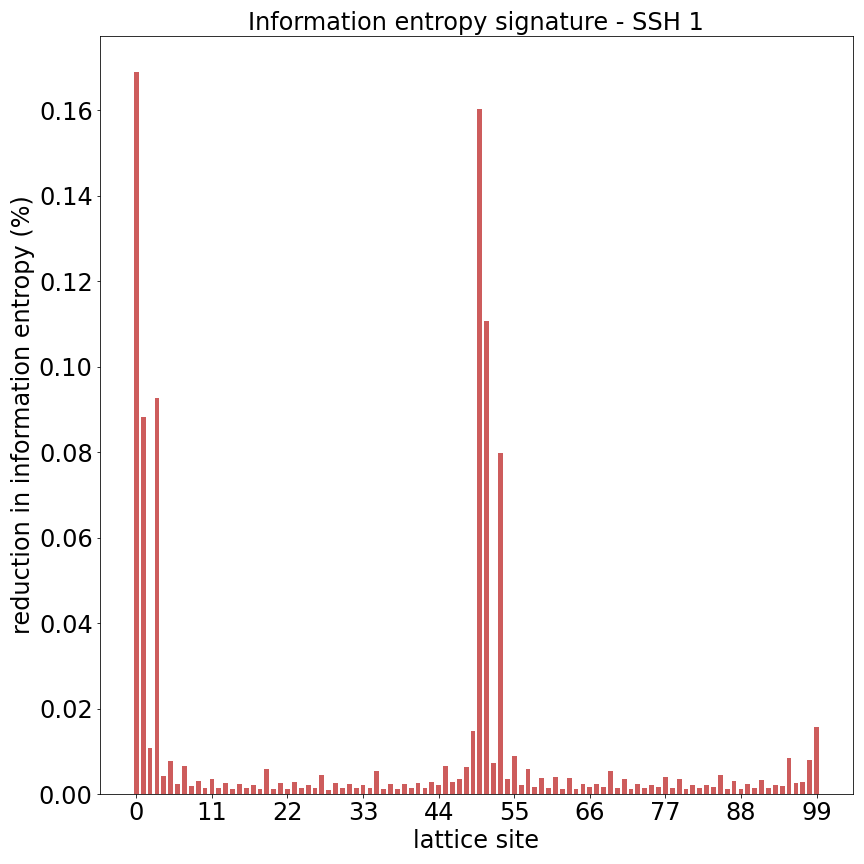
\includegraphics[width=0.49\textwidth]{./ssh1/periodic_100_6561/plot_feature_importances.png}}\quad
\subfigure[]{\label{feature_importances_ssh2}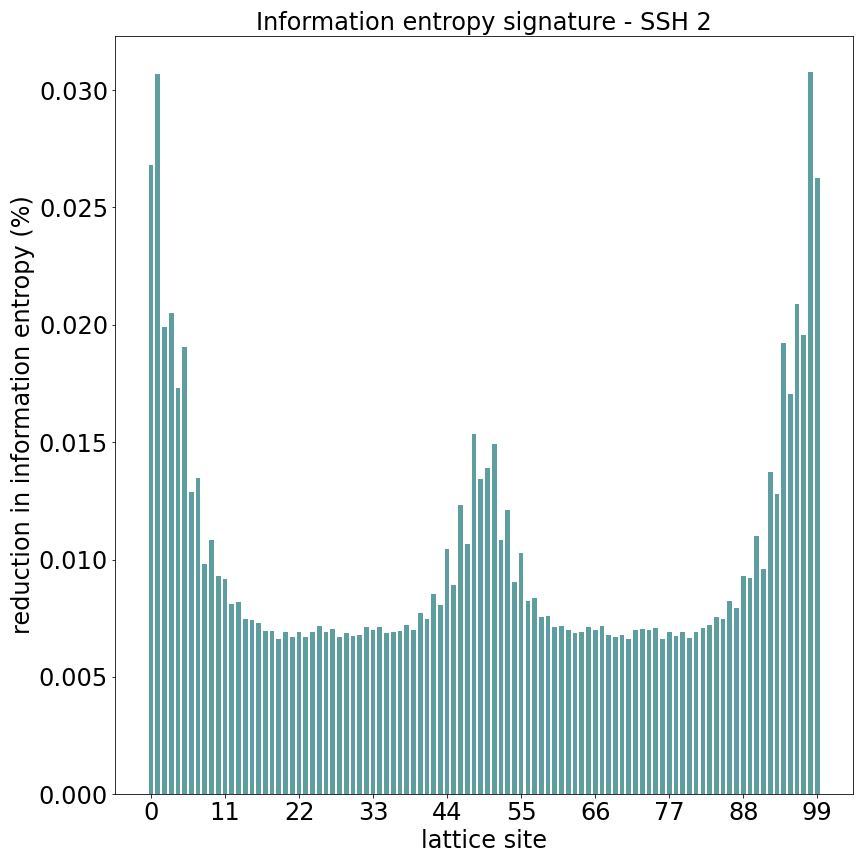
\includegraphics[width=0.49\textwidth]{./ssh2/periodic_100_6561/plot_feature_importances.png}}\quad
\caption{Information entropy signatures of the topological phase transitions obtained from the numerical experiments described in section \ref{numerical_experiments}. (a) In experiment 1 (section \ref{experiment_1}), the two sharp peaks in the Shannon entropy signal account for approximately 70\% of reduction in information entropy. These two peaks correspond to the lattice sites $S_1$. (b) In experiment 2 (section \ref{experiment_2}), the three visible peaks account for approximately 30\% of reduction in information entropy. These three peaks are located along lattice sites $S_2$.}
\label{feature_importances}
\end{figure}

%\begin{figure}
%\centering
%\subfigure[]{\label{fourier_feature_importances_ssh1}\includegraphics[width=0.49\textwidth]{./ssh1/periodic_100_6561/%plot_fourier_feature_importances.png}}\quad
%\subfigure[]{\label{fourier_feature_importances_ssh2}\includegraphics[width=0.49\textwidth]{./ssh2/periodic_100_6561/%plot_fourier_feature_importances.png}}\quad
%\caption{Information entropy signatures of the topological phase transitions obtained from the numerical experiments described in section %%\ref{numerical_experiments}. (a) In experiment 1 (section \ref{experiment_1}), the two sharp peaks in the Shannon entropy signal account for %approximately 70\% of reduction in information entropy. These two peaks correspond to the lattice sites $S_1$. (b) In experiment 2 (section \ref{experiment_2}), the three visible peaks account for approximately 30\% of reduction in information entropy. These three peaks are located %along lattice sites $S_2$.}
%\label{fourier_feature_importances}
%\end{figure}

\citequote{motif_real_space}

%merlin.mbs apsrev4-1.bst 2010-07-25 4.21a (PWD, AO, DPC) hacked
%Control: key (0)
%Control: author (8) initials jnrlst
%Control: editor formatted (1) identically to author
%Control: production of article title (-1) disabled
%Control: page (0) single
%Control: year (1) truncated
%Control: production of eprint (0) enabled
\begin{thebibliography}{56}%
\makeatletter
\providecommand \@ifxundefined [1]{%
 \@ifx{#1\undefined}
}%
\providecommand \@ifnum [1]{%
 \ifnum #1\expandafter \@firstoftwo
 \else \expandafter \@secondoftwo
 \fi
}%
\providecommand \@ifx [1]{%
 \ifx #1\expandafter \@firstoftwo
 \else \expandafter \@secondoftwo
 \fi
}%
\providecommand \natexlab [1]{#1}%
\providecommand \enquote  [1]{``#1''}%
\providecommand \bibnamefont  [1]{#1}%
\providecommand \bibfnamefont [1]{#1}%
\providecommand \citenamefont [1]{#1}%
\providecommand \href@noop [0]{\@secondoftwo}%
\providecommand \href [0]{\begingroup \@sanitize@url \@href}%
\providecommand \@href[1]{\@@startlink{#1}\@@href}%
\providecommand \@@href[1]{\endgroup#1\@@endlink}%
\providecommand \@sanitize@url [0]{\catcode `\\12\catcode `\$12\catcode
  `\&12\catcode `\#12\catcode `\^12\catcode `\_12\catcode `\%12\relax}%
\providecommand \@@startlink[1]{}%
\providecommand \@@endlink[0]{}%
\providecommand \url  [0]{\begingroup\@sanitize@url \@url }%
\providecommand \@url [1]{\endgroup\@href {#1}{\urlprefix }}%
\providecommand \urlprefix  [0]{URL }%
\providecommand \Eprint [0]{\href }%
\providecommand \doibase [0]{http://dx.doi.org/}%
\providecommand \selectlanguage [0]{\@gobble}%
\providecommand \bibinfo  [0]{\@secondoftwo}%
\providecommand \bibfield  [0]{\@secondoftwo}%
\providecommand \translation [1]{[#1]}%
\providecommand \BibitemOpen [0]{}%
\providecommand \bibitemStop [0]{}%
\providecommand \bibitemNoStop [0]{.\EOS\space}%
\providecommand \EOS [0]{\spacefactor3000\relax}%
\providecommand \BibitemShut  [1]{\csname bibitem#1\endcsname}%
\let\auto@bib@innerbib\@empty
%</preamble>
\bibitem [{\citenamefont {Hasan}\ and\ \citenamefont
  {Kane}(2010)}]{RevModPhys.82.3045}%
  \BibitemOpen
  \bibfield  {author} {\bibinfo {author} {\bibfnamefont {M.~Z.}\ \bibnamefont
  {Hasan}}\ and\ \bibinfo {author} {\bibfnamefont {C.~L.}\ \bibnamefont
  {Kane}},\ }\href@noop {} {\bibfield  {journal} {\bibinfo  {journal} {Rev.
  Mod. Phys.}\ }\textbf {\bibinfo {volume} {82}},\ \bibinfo {pages} {3045}
  (\bibinfo {year} {2010})}\BibitemShut {NoStop}%
\bibitem [{\citenamefont {Continentino}(2017)}]{CONTINENTINO2017A1}%
  \BibitemOpen
  \bibfield  {author} {\bibinfo {author} {\bibfnamefont {M.~A.}\ \bibnamefont
  {Continentino}},\ }\href@noop {} {\bibfield  {journal} {\bibinfo  {journal}
  {Physica B: Condensed Matter}\ }\textbf {\bibinfo {volume} {505}},\ \bibinfo
  {pages} {A1 } (\bibinfo {year} {2017})}\BibitemShut {NoStop}%
\bibitem [{\citenamefont {Puel}\ \emph {et~al.}(2017)\citenamefont {Puel},
  \citenamefont {Sacramento},\ and\ \citenamefont
  {Continentino}}]{PhysRevB.95.094509}%
  \BibitemOpen
  \bibfield  {author} {\bibinfo {author} {\bibfnamefont {T.~O.}\ \bibnamefont
  {Puel}}, \bibinfo {author} {\bibfnamefont {P.~D.}\ \bibnamefont
  {Sacramento}}, \ and\ \bibinfo {author} {\bibfnamefont {M.~A.}\ \bibnamefont
  {Continentino}},\ }\href@noop {} {\bibfield  {journal} {\bibinfo  {journal}
  {Phys. Rev. B}\ }\textbf {\bibinfo {volume} {95}},\ \bibinfo {pages} {094509}
  (\bibinfo {year} {2017})}\BibitemShut {NoStop}%
\bibitem [{\citenamefont {Griffith}\ and\ \citenamefont
  {Continentino}(2018)}]{PhysRevE.97.012107}%
  \BibitemOpen
  \bibfield  {author} {\bibinfo {author} {\bibfnamefont {M.~A.}\ \bibnamefont
  {Griffith}}\ and\ \bibinfo {author} {\bibfnamefont {M.~A.}\ \bibnamefont
  {Continentino}},\ }\href@noop {} {\bibfield  {journal} {\bibinfo  {journal}
  {Phys. Rev. E}\ }\textbf {\bibinfo {volume} {97}},\ \bibinfo {pages} {012107}
  (\bibinfo {year} {2018})}\BibitemShut {NoStop}%
\bibitem [{\citenamefont {Ryu}\ \emph {et~al.}(2010)\citenamefont {Ryu},
  \citenamefont {Schnyder}, \citenamefont {Furusaki},\ and\ \citenamefont
  {Ludwig}}]{ryu2010topological}%
  \BibitemOpen
  \bibfield  {author} {\bibinfo {author} {\bibfnamefont {S.}~\bibnamefont
  {Ryu}}, \bibinfo {author} {\bibfnamefont {A.~P.}\ \bibnamefont {Schnyder}},
  \bibinfo {author} {\bibfnamefont {A.}~\bibnamefont {Furusaki}}, \ and\
  \bibinfo {author} {\bibfnamefont {A.~W.}\ \bibnamefont {Ludwig}},\
  }\href@noop {} {\bibfield  {journal} {\bibinfo  {journal} {New Journal of
  Physics}\ }\textbf {\bibinfo {volume} {12}},\ \bibinfo {pages} {065010}
  (\bibinfo {year} {2010})}\BibitemShut {NoStop}%
\bibitem [{\citenamefont {Atala}\ \emph {et~al.}(2013)\citenamefont {Atala},
  \citenamefont {Aidelsburger}, \citenamefont {Barreiro}, \citenamefont
  {Abanin}, \citenamefont {Kitagawa}, \citenamefont {Demler},\ and\
  \citenamefont {Bloch}}]{atala2013direct}%
  \BibitemOpen
  \bibfield  {author} {\bibinfo {author} {\bibfnamefont {M.}~\bibnamefont
  {Atala}}, \bibinfo {author} {\bibfnamefont {M.}~\bibnamefont {Aidelsburger}},
  \bibinfo {author} {\bibfnamefont {J.~T.}\ \bibnamefont {Barreiro}}, \bibinfo
  {author} {\bibfnamefont {D.}~\bibnamefont {Abanin}}, \bibinfo {author}
  {\bibfnamefont {T.}~\bibnamefont {Kitagawa}}, \bibinfo {author}
  {\bibfnamefont {E.}~\bibnamefont {Demler}}, \ and\ \bibinfo {author}
  {\bibfnamefont {I.}~\bibnamefont {Bloch}},\ }\href@noop {} {\bibfield
  {journal} {\bibinfo  {journal} {Nature Physics}\ }\textbf {\bibinfo {volume}
  {9}},\ \bibinfo {pages} {795} (\bibinfo {year} {2013})}\BibitemShut {NoStop}%
\bibitem [{\citenamefont {Stuhl}\ \emph {et~al.}(2015)\citenamefont {Stuhl},
  \citenamefont {Lu}, \citenamefont {Aycock}, \citenamefont {Genkina},\ and\
  \citenamefont {Spielman}}]{Stuhl1514}%
  \BibitemOpen
  \bibfield  {author} {\bibinfo {author} {\bibfnamefont {B.~K.}\ \bibnamefont
  {Stuhl}}, \bibinfo {author} {\bibfnamefont {H.-I.}\ \bibnamefont {Lu}},
  \bibinfo {author} {\bibfnamefont {L.~M.}\ \bibnamefont {Aycock}}, \bibinfo
  {author} {\bibfnamefont {D.}~\bibnamefont {Genkina}}, \ and\ \bibinfo
  {author} {\bibfnamefont {I.~B.}\ \bibnamefont {Spielman}},\ }\href@noop {}
  {\bibfield  {journal} {\bibinfo  {journal} {Science}\ }\textbf {\bibinfo
  {volume} {349}},\ \bibinfo {pages} {1514} (\bibinfo {year}
  {2015})}\BibitemShut {NoStop}%
\bibitem [{\citenamefont {Leder}\ \emph {et~al.}(2016)\citenamefont {Leder},
  \citenamefont {Grossert}, \citenamefont {Sitta}, \citenamefont {Genske},
  \citenamefont {Rosch},\ and\ \citenamefont {Weitz}}]{leder2016real}%
  \BibitemOpen
  \bibfield  {author} {\bibinfo {author} {\bibfnamefont {M.}~\bibnamefont
  {Leder}}, \bibinfo {author} {\bibfnamefont {C.}~\bibnamefont {Grossert}},
  \bibinfo {author} {\bibfnamefont {L.}~\bibnamefont {Sitta}}, \bibinfo
  {author} {\bibfnamefont {M.}~\bibnamefont {Genske}}, \bibinfo {author}
  {\bibfnamefont {A.}~\bibnamefont {Rosch}}, \ and\ \bibinfo {author}
  {\bibfnamefont {M.}~\bibnamefont {Weitz}},\ }\href@noop {} {\bibfield
  {journal} {\bibinfo  {journal} {Nature communications}\ }\textbf {\bibinfo
  {volume} {7}},\ \bibinfo {pages} {13112} (\bibinfo {year}
  {2016})}\BibitemShut {NoStop}%
\bibitem [{\citenamefont {Goldman}\ \emph {et~al.}(2016)\citenamefont
  {Goldman}, \citenamefont {Budich},\ and\ \citenamefont
  {Zoller}}]{goldman2016topological}%
  \BibitemOpen
  \bibfield  {author} {\bibinfo {author} {\bibfnamefont {N.}~\bibnamefont
  {Goldman}}, \bibinfo {author} {\bibfnamefont {J.}~\bibnamefont {Budich}}, \
  and\ \bibinfo {author} {\bibfnamefont {P.}~\bibnamefont {Zoller}},\
  }\href@noop {} {\bibfield  {journal} {\bibinfo  {journal} {Nature Physics}\
  }\textbf {\bibinfo {volume} {12}},\ \bibinfo {pages} {639} (\bibinfo {year}
  {2016})}\BibitemShut {NoStop}%
\bibitem [{\citenamefont {Meier}\ \emph {et~al.}(2016)\citenamefont {Meier},
  \citenamefont {An},\ and\ \citenamefont {Gadway}}]{meier2016observation}%
  \BibitemOpen
  \bibfield  {author} {\bibinfo {author} {\bibfnamefont {E.~J.}\ \bibnamefont
  {Meier}}, \bibinfo {author} {\bibfnamefont {F.~A.}\ \bibnamefont {An}}, \
  and\ \bibinfo {author} {\bibfnamefont {B.}~\bibnamefont {Gadway}},\
  }\href@noop {} {\bibfield  {journal} {\bibinfo  {journal} {Nature
  communications}\ }\textbf {\bibinfo {volume} {7}},\ \bibinfo {pages} {13986}
  (\bibinfo {year} {2016})}\BibitemShut {NoStop}%
\bibitem [{\citenamefont {Hafezi}\ \emph {et~al.}(2013)\citenamefont {Hafezi},
  \citenamefont {Mittal}, \citenamefont {Fan}, \citenamefont {Migdall},\ and\
  \citenamefont {Taylor}}]{hafezi2013imaging}%
  \BibitemOpen
  \bibfield  {author} {\bibinfo {author} {\bibfnamefont {M.}~\bibnamefont
  {Hafezi}}, \bibinfo {author} {\bibfnamefont {S.}~\bibnamefont {Mittal}},
  \bibinfo {author} {\bibfnamefont {J.}~\bibnamefont {Fan}}, \bibinfo {author}
  {\bibfnamefont {A.}~\bibnamefont {Migdall}}, \ and\ \bibinfo {author}
  {\bibfnamefont {J.}~\bibnamefont {Taylor}},\ }\href@noop {} {\bibfield
  {journal} {\bibinfo  {journal} {Nature Photonics}\ }\textbf {\bibinfo
  {volume} {7}},\ \bibinfo {pages} {1001} (\bibinfo {year} {2013})}\BibitemShut
  {NoStop}%
\bibitem [{\citenamefont {Lu}\ \emph {et~al.}(2016)\citenamefont {Lu},
  \citenamefont {Joannopoulos},\ and\ \citenamefont
  {Solja{\v{c}}i{\'c}}}]{lu2016topological}%
  \BibitemOpen
  \bibfield  {author} {\bibinfo {author} {\bibfnamefont {L.}~\bibnamefont
  {Lu}}, \bibinfo {author} {\bibfnamefont {J.~D.}\ \bibnamefont
  {Joannopoulos}}, \ and\ \bibinfo {author} {\bibfnamefont {M.}~\bibnamefont
  {Solja{\v{c}}i{\'c}}},\ }\href@noop {} {\bibfield  {journal} {\bibinfo
  {journal} {Nature Physics}\ }\textbf {\bibinfo {volume} {12}},\ \bibinfo
  {pages} {626} (\bibinfo {year} {2016})}\BibitemShut {NoStop}%
\bibitem [{\citenamefont {Peano}\ \emph {et~al.}(2015)\citenamefont {Peano},
  \citenamefont {Brendel}, \citenamefont {Schmidt},\ and\ \citenamefont
  {Marquardt}}]{PhysRevX.5.031011}%
  \BibitemOpen
  \bibfield  {author} {\bibinfo {author} {\bibfnamefont {V.}~\bibnamefont
  {Peano}}, \bibinfo {author} {\bibfnamefont {C.}~\bibnamefont {Brendel}},
  \bibinfo {author} {\bibfnamefont {M.}~\bibnamefont {Schmidt}}, \ and\
  \bibinfo {author} {\bibfnamefont {F.}~\bibnamefont {Marquardt}},\ }\href@noop
  {} {\bibfield  {journal} {\bibinfo  {journal} {Phys. Rev. X}\ }\textbf
  {\bibinfo {volume} {5}},\ \bibinfo {pages} {031011} (\bibinfo {year}
  {2015})}\BibitemShut {NoStop}%
\bibitem [{\citenamefont {Kitagawa}\ \emph {et~al.}(2012)\citenamefont
  {Kitagawa}, \citenamefont {Broome}, \citenamefont {Fedrizzi}, \citenamefont
  {Rudner}, \citenamefont {Berg}, \citenamefont {Kassal}, \citenamefont
  {Aspuru-Guzik}, \citenamefont {Demler},\ and\ \citenamefont
  {White}}]{kitagawa2012observation}%
  \BibitemOpen
  \bibfield  {author} {\bibinfo {author} {\bibfnamefont {T.}~\bibnamefont
  {Kitagawa}}, \bibinfo {author} {\bibfnamefont {M.~A.}\ \bibnamefont
  {Broome}}, \bibinfo {author} {\bibfnamefont {A.}~\bibnamefont {Fedrizzi}},
  \bibinfo {author} {\bibfnamefont {M.~S.}\ \bibnamefont {Rudner}}, \bibinfo
  {author} {\bibfnamefont {E.}~\bibnamefont {Berg}}, \bibinfo {author}
  {\bibfnamefont {I.}~\bibnamefont {Kassal}}, \bibinfo {author} {\bibfnamefont
  {A.}~\bibnamefont {Aspuru-Guzik}}, \bibinfo {author} {\bibfnamefont
  {E.}~\bibnamefont {Demler}}, \ and\ \bibinfo {author} {\bibfnamefont {A.~G.}\
  \bibnamefont {White}},\ }\href@noop {} {\bibfield  {journal} {\bibinfo
  {journal} {Nature communications}\ }\textbf {\bibinfo {volume} {3}},\
  \bibinfo {pages} {882} (\bibinfo {year} {2012})}\BibitemShut {NoStop}%
\bibitem [{\citenamefont {Cardano}\ \emph {et~al.}(2016)\citenamefont
  {Cardano}, \citenamefont {Maffei}, \citenamefont {Massa}, \citenamefont
  {Piccirillo}, \citenamefont {De~Lisio}, \citenamefont {De~Filippis},
  \citenamefont {Cataudella}, \citenamefont {Santamato},\ and\ \citenamefont
  {Marrucci}}]{cardano2016statistical}%
  \BibitemOpen
  \bibfield  {author} {\bibinfo {author} {\bibfnamefont {F.}~\bibnamefont
  {Cardano}}, \bibinfo {author} {\bibfnamefont {M.}~\bibnamefont {Maffei}},
  \bibinfo {author} {\bibfnamefont {F.}~\bibnamefont {Massa}}, \bibinfo
  {author} {\bibfnamefont {B.}~\bibnamefont {Piccirillo}}, \bibinfo {author}
  {\bibfnamefont {C.}~\bibnamefont {De~Lisio}}, \bibinfo {author}
  {\bibfnamefont {G.}~\bibnamefont {De~Filippis}}, \bibinfo {author}
  {\bibfnamefont {V.}~\bibnamefont {Cataudella}}, \bibinfo {author}
  {\bibfnamefont {E.}~\bibnamefont {Santamato}}, \ and\ \bibinfo {author}
  {\bibfnamefont {L.}~\bibnamefont {Marrucci}},\ }\href@noop {} {\bibfield
  {journal} {\bibinfo  {journal} {Nature communications}\ }\textbf {\bibinfo
  {volume} {7}},\ \bibinfo {pages} {11439} (\bibinfo {year}
  {2016})}\BibitemShut {NoStop}%
\bibitem [{\citenamefont {Flurin}\ \emph {et~al.}(2017)\citenamefont {Flurin},
  \citenamefont {Ramasesh}, \citenamefont {Hacohen-Gourgy}, \citenamefont
  {Martin}, \citenamefont {Yao},\ and\ \citenamefont
  {Siddiqi}}]{PhysRevX.7.031023}%
  \BibitemOpen
  \bibfield  {author} {\bibinfo {author} {\bibfnamefont {E.}~\bibnamefont
  {Flurin}}, \bibinfo {author} {\bibfnamefont {V.~V.}\ \bibnamefont
  {Ramasesh}}, \bibinfo {author} {\bibfnamefont {S.}~\bibnamefont
  {Hacohen-Gourgy}}, \bibinfo {author} {\bibfnamefont {L.~S.}\ \bibnamefont
  {Martin}}, \bibinfo {author} {\bibfnamefont {N.~Y.}\ \bibnamefont {Yao}}, \
  and\ \bibinfo {author} {\bibfnamefont {I.}~\bibnamefont {Siddiqi}},\
  }\href@noop {} {\bibfield  {journal} {\bibinfo  {journal} {Phys. Rev. X}\
  }\textbf {\bibinfo {volume} {7}},\ \bibinfo {pages} {031023} (\bibinfo {year}
  {2017})}\BibitemShut {NoStop}%
\bibitem [{\citenamefont {Soluyanov}\ \emph {et~al.}(2015)\citenamefont
  {Soluyanov}, \citenamefont {Gresch}, \citenamefont {Wang}, \citenamefont
  {Wu}, \citenamefont {Troyer}, \citenamefont {Dai},\ and\ \citenamefont
  {Bernevig}}]{soluyanov2015type}%
  \BibitemOpen
  \bibfield  {author} {\bibinfo {author} {\bibfnamefont {A.~A.}\ \bibnamefont
  {Soluyanov}}, \bibinfo {author} {\bibfnamefont {D.}~\bibnamefont {Gresch}},
  \bibinfo {author} {\bibfnamefont {Z.}~\bibnamefont {Wang}}, \bibinfo {author}
  {\bibfnamefont {Q.}~\bibnamefont {Wu}}, \bibinfo {author} {\bibfnamefont
  {M.}~\bibnamefont {Troyer}}, \bibinfo {author} {\bibfnamefont
  {X.}~\bibnamefont {Dai}}, \ and\ \bibinfo {author} {\bibfnamefont {B.~A.}\
  \bibnamefont {Bernevig}},\ }\href@noop {} {\bibfield  {journal} {\bibinfo
  {journal} {Nature}\ }\textbf {\bibinfo {volume} {527}},\ \bibinfo {pages}
  {495} (\bibinfo {year} {2015})}\BibitemShut {NoStop}%
\bibitem [{\citenamefont {Lv}\ \emph {et~al.}(2015)\citenamefont {Lv},
  \citenamefont {Weng}, \citenamefont {Fu}, \citenamefont {Wang}, \citenamefont
  {Miao}, \citenamefont {Ma}, \citenamefont {Richard}, \citenamefont {Huang},
  \citenamefont {Zhao}, \citenamefont {Chen}, \citenamefont {Fang},
  \citenamefont {Dai}, \citenamefont {Qian},\ and\ \citenamefont
  {Ding}}]{PhysRevX.5.031013}%
  \BibitemOpen
  \bibfield  {author} {\bibinfo {author} {\bibfnamefont {B.~Q.}\ \bibnamefont
  {Lv}}, \bibinfo {author} {\bibfnamefont {H.~M.}\ \bibnamefont {Weng}},
  \bibinfo {author} {\bibfnamefont {B.~B.}\ \bibnamefont {Fu}}, \bibinfo
  {author} {\bibfnamefont {X.~P.}\ \bibnamefont {Wang}}, \bibinfo {author}
  {\bibfnamefont {H.}~\bibnamefont {Miao}}, \bibinfo {author} {\bibfnamefont
  {J.}~\bibnamefont {Ma}}, \bibinfo {author} {\bibfnamefont {P.}~\bibnamefont
  {Richard}}, \bibinfo {author} {\bibfnamefont {X.~C.}\ \bibnamefont {Huang}},
  \bibinfo {author} {\bibfnamefont {L.~X.}\ \bibnamefont {Zhao}}, \bibinfo
  {author} {\bibfnamefont {G.~F.}\ \bibnamefont {Chen}}, \bibinfo {author}
  {\bibfnamefont {Z.}~\bibnamefont {Fang}}, \bibinfo {author} {\bibfnamefont
  {X.}~\bibnamefont {Dai}}, \bibinfo {author} {\bibfnamefont {T.}~\bibnamefont
  {Qian}}, \ and\ \bibinfo {author} {\bibfnamefont {H.}~\bibnamefont {Ding}},\
  }\href@noop {} {\bibfield  {journal} {\bibinfo  {journal} {Phys. Rev. X}\
  }\textbf {\bibinfo {volume} {5}},\ \bibinfo {pages} {031013} (\bibinfo {year}
  {2015})}\BibitemShut {NoStop}%
\bibitem [{\citenamefont {Su}\ \emph {et~al.}(1979)\citenamefont {Su},
  \citenamefont {Schrieffer},\ and\ \citenamefont
  {Heeger}}]{PhysRevLett.42.1698}%
  \BibitemOpen
  \bibfield  {author} {\bibinfo {author} {\bibfnamefont {W.~P.}\ \bibnamefont
  {Su}}, \bibinfo {author} {\bibfnamefont {J.~R.}\ \bibnamefont {Schrieffer}},
  \ and\ \bibinfo {author} {\bibfnamefont {A.~J.}\ \bibnamefont {Heeger}},\
  }\href@noop {} {\bibfield  {journal} {\bibinfo  {journal} {Phys. Rev. Lett.}\
  }\textbf {\bibinfo {volume} {42}},\ \bibinfo {pages} {1698} (\bibinfo {year}
  {1979})}\BibitemShut {NoStop}%
\bibitem [{\citenamefont {Maffei}\ \emph {et~al.}(2018)\citenamefont {Maffei},
  \citenamefont {Dauphin}, \citenamefont {Cardano}, \citenamefont
  {Lewenstein},\ and\ \citenamefont {Massignan}}]{maffei2018topological}%
  \BibitemOpen
  \bibfield  {author} {\bibinfo {author} {\bibfnamefont {M.}~\bibnamefont
  {Maffei}}, \bibinfo {author} {\bibfnamefont {A.}~\bibnamefont {Dauphin}},
  \bibinfo {author} {\bibfnamefont {F.}~\bibnamefont {Cardano}}, \bibinfo
  {author} {\bibfnamefont {M.}~\bibnamefont {Lewenstein}}, \ and\ \bibinfo
  {author} {\bibfnamefont {P.}~\bibnamefont {Massignan}},\ }\href@noop {}
  {\bibfield  {journal} {\bibinfo  {journal} {New Journal of Physics}\ }\textbf
  {\bibinfo {volume} {20}},\ \bibinfo {pages} {013023} (\bibinfo {year}
  {2018})}\BibitemShut {NoStop}%
\bibitem [{\citenamefont {Heeger}(2001)}]{RevModPhys.73.681}%
  \BibitemOpen
  \bibfield  {author} {\bibinfo {author} {\bibfnamefont {A.~J.}\ \bibnamefont
  {Heeger}},\ }\href@noop {} {\bibfield  {journal} {\bibinfo  {journal} {Rev.
  Mod. Phys.}\ }\textbf {\bibinfo {volume} {73}},\ \bibinfo {pages} {681}
  (\bibinfo {year} {2001})}\BibitemShut {NoStop}%
\bibitem [{\citenamefont {Kane}\ and\ \citenamefont
  {Lubensky}(2014)}]{kane2014topological}%
  \BibitemOpen
  \bibfield  {author} {\bibinfo {author} {\bibfnamefont {C.}~\bibnamefont
  {Kane}}\ and\ \bibinfo {author} {\bibfnamefont {T.}~\bibnamefont
  {Lubensky}},\ }\href@noop {} {\bibfield  {journal} {\bibinfo  {journal}
  {Nature Physics}\ }\textbf {\bibinfo {volume} {10}},\ \bibinfo {pages} {39}
  (\bibinfo {year} {2014})}\BibitemShut {NoStop}%
\bibitem [{\citenamefont {Chen}\ \emph {et~al.}(2014)\citenamefont {Chen},
  \citenamefont {Upadhyaya},\ and\ \citenamefont {Vitelli}}]{Chen13004}%
  \BibitemOpen
  \bibfield  {author} {\bibinfo {author} {\bibfnamefont {B.~G.-g.}\
  \bibnamefont {Chen}}, \bibinfo {author} {\bibfnamefont {N.}~\bibnamefont
  {Upadhyaya}}, \ and\ \bibinfo {author} {\bibfnamefont {V.}~\bibnamefont
  {Vitelli}},\ }\href@noop {} {\bibfield  {journal} {\bibinfo  {journal}
  {Proceedings of the National Academy of Sciences}\ }\textbf {\bibinfo
  {volume} {111}},\ \bibinfo {pages} {13004} (\bibinfo {year}
  {2014})}\BibitemShut {NoStop}%
\bibitem [{\citenamefont {Carrasquilla}\ and\ \citenamefont
  {Melko}(2017)}]{carrasquilla2017machine}%
  \BibitemOpen
  \bibfield  {author} {\bibinfo {author} {\bibfnamefont {J.}~\bibnamefont
  {Carrasquilla}}\ and\ \bibinfo {author} {\bibfnamefont {R.~G.}\ \bibnamefont
  {Melko}},\ }\href@noop {} {\bibfield  {journal} {\bibinfo  {journal} {Nature
  Physics}\ }\textbf {\bibinfo {volume} {13}},\ \bibinfo {pages} {431}
  (\bibinfo {year} {2017})}\BibitemShut {NoStop}%
\bibitem [{\citenamefont {Ch'ng}\ \emph {et~al.}(2017)\citenamefont {Ch'ng},
  \citenamefont {Carrasquilla}, \citenamefont {Melko},\ and\ \citenamefont
  {Khatami}}]{PhysRevX.7.031038}%
  \BibitemOpen
  \bibfield  {author} {\bibinfo {author} {\bibfnamefont {K.}~\bibnamefont
  {Ch'ng}}, \bibinfo {author} {\bibfnamefont {J.}~\bibnamefont {Carrasquilla}},
  \bibinfo {author} {\bibfnamefont {R.~G.}\ \bibnamefont {Melko}}, \ and\
  \bibinfo {author} {\bibfnamefont {E.}~\bibnamefont {Khatami}},\ }\href@noop
  {} {\bibfield  {journal} {\bibinfo  {journal} {Phys. Rev. X}\ }\textbf
  {\bibinfo {volume} {7}},\ \bibinfo {pages} {031038} (\bibinfo {year}
  {2017})}\BibitemShut {NoStop}%
\bibitem [{\citenamefont {Wang}(2016)}]{PhysRevB.94.195105}%
  \BibitemOpen
  \bibfield  {author} {\bibinfo {author} {\bibfnamefont {L.}~\bibnamefont
  {Wang}},\ }\href@noop {} {\bibfield  {journal} {\bibinfo  {journal} {Phys.
  Rev. B}\ }\textbf {\bibinfo {volume} {94}},\ \bibinfo {pages} {195105}
  (\bibinfo {year} {2016})}\BibitemShut {NoStop}%
\bibitem [{\citenamefont {Broecker}\ \emph {et~al.}(2017)\citenamefont
  {Broecker}, \citenamefont {Carrasquilla}, \citenamefont {Melko},\ and\
  \citenamefont {Trebst}}]{broecker2017machine}%
  \BibitemOpen
  \bibfield  {author} {\bibinfo {author} {\bibfnamefont {P.}~\bibnamefont
  {Broecker}}, \bibinfo {author} {\bibfnamefont {J.}~\bibnamefont
  {Carrasquilla}}, \bibinfo {author} {\bibfnamefont {R.~G.}\ \bibnamefont
  {Melko}}, \ and\ \bibinfo {author} {\bibfnamefont {S.}~\bibnamefont
  {Trebst}},\ }\href@noop {} {\bibfield  {journal} {\bibinfo  {journal}
  {Scientific reports}\ }\textbf {\bibinfo {volume} {7}},\ \bibinfo {pages}
  {8823} (\bibinfo {year} {2017})}\BibitemShut {NoStop}%
\bibitem [{\citenamefont {Van~Nieuwenburg}\ \emph {et~al.}(2017)\citenamefont
  {Van~Nieuwenburg}, \citenamefont {Liu},\ and\ \citenamefont
  {Huber}}]{van2017learning}%
  \BibitemOpen
  \bibfield  {author} {\bibinfo {author} {\bibfnamefont {E.~P.}\ \bibnamefont
  {Van~Nieuwenburg}}, \bibinfo {author} {\bibfnamefont {Y.-H.}\ \bibnamefont
  {Liu}}, \ and\ \bibinfo {author} {\bibfnamefont {S.~D.}\ \bibnamefont
  {Huber}},\ }\href@noop {} {\bibfield  {journal} {\bibinfo  {journal} {Nature
  Physics}\ }\textbf {\bibinfo {volume} {13}},\ \bibinfo {pages} {435}
  (\bibinfo {year} {2017})}\BibitemShut {NoStop}%
\bibitem [{\citenamefont {Zhang}\ \emph {et~al.}(2018)\citenamefont {Zhang},
  \citenamefont {Shen},\ and\ \citenamefont {Zhai}}]{PhysRevLett.120.066401}%
  \BibitemOpen
  \bibfield  {author} {\bibinfo {author} {\bibfnamefont {P.}~\bibnamefont
  {Zhang}}, \bibinfo {author} {\bibfnamefont {H.}~\bibnamefont {Shen}}, \ and\
  \bibinfo {author} {\bibfnamefont {H.}~\bibnamefont {Zhai}},\ }\href@noop {}
  {\bibfield  {journal} {\bibinfo  {journal} {Phys. Rev. Lett.}\ }\textbf
  {\bibinfo {volume} {120}},\ \bibinfo {pages} {066401} (\bibinfo {year}
  {2018})}\BibitemShut {NoStop}%
\bibitem [{\citenamefont {Sun}\ \emph {et~al.}(2018)\citenamefont {Sun},
  \citenamefont {Yi}, \citenamefont {Zhang}, \citenamefont {Shen},\ and\
  \citenamefont {Zhai}}]{PhysRevB.98.085402}%
  \BibitemOpen
  \bibfield  {author} {\bibinfo {author} {\bibfnamefont {N.}~\bibnamefont
  {Sun}}, \bibinfo {author} {\bibfnamefont {J.}~\bibnamefont {Yi}}, \bibinfo
  {author} {\bibfnamefont {P.}~\bibnamefont {Zhang}}, \bibinfo {author}
  {\bibfnamefont {H.}~\bibnamefont {Shen}}, \ and\ \bibinfo {author}
  {\bibfnamefont {H.}~\bibnamefont {Zhai}},\ }\href@noop {} {\bibfield
  {journal} {\bibinfo  {journal} {Phys. Rev. B}\ }\textbf {\bibinfo {volume}
  {98}},\ \bibinfo {pages} {085402} (\bibinfo {year} {2018})}\BibitemShut
  {NoStop}%
\bibitem [{\citenamefont {Suchsland}\ and\ \citenamefont
  {Wessel}(2018)}]{PhysRevB.97.174435}%
  \BibitemOpen
  \bibfield  {author} {\bibinfo {author} {\bibfnamefont {P.}~\bibnamefont
  {Suchsland}}\ and\ \bibinfo {author} {\bibfnamefont {S.}~\bibnamefont
  {Wessel}},\ }\href@noop {} {\bibfield  {journal} {\bibinfo  {journal} {Phys.
  Rev. B}\ }\textbf {\bibinfo {volume} {97}},\ \bibinfo {pages} {174435}
  (\bibinfo {year} {2018})}\BibitemShut {NoStop}%
\bibitem [{\citenamefont {Zhang}\ and\ \citenamefont
  {Kim}(2017)}]{PhysRevLett.118.216401}%
  \BibitemOpen
  \bibfield  {author} {\bibinfo {author} {\bibfnamefont {Y.}~\bibnamefont
  {Zhang}}\ and\ \bibinfo {author} {\bibfnamefont {E.-A.}\ \bibnamefont
  {Kim}},\ }\href@noop {} {\bibfield  {journal} {\bibinfo  {journal} {Phys.
  Rev. Lett.}\ }\textbf {\bibinfo {volume} {118}},\ \bibinfo {pages} {216401}
  (\bibinfo {year} {2017})}\BibitemShut {NoStop}%
\bibitem [{\citenamefont {Venderley}\ \emph {et~al.}(2018)\citenamefont
  {Venderley}, \citenamefont {Khemani},\ and\ \citenamefont
  {Kim}}]{PhysRevLett.120.257204}%
  \BibitemOpen
  \bibfield  {author} {\bibinfo {author} {\bibfnamefont {J.}~\bibnamefont
  {Venderley}}, \bibinfo {author} {\bibfnamefont {V.}~\bibnamefont {Khemani}},
  \ and\ \bibinfo {author} {\bibfnamefont {E.-A.}\ \bibnamefont {Kim}},\
  }\href@noop {} {\bibfield  {journal} {\bibinfo  {journal} {Phys. Rev. Lett.}\
  }\textbf {\bibinfo {volume} {120}},\ \bibinfo {pages} {257204} (\bibinfo
  {year} {2018})}\BibitemShut {NoStop}%
\bibitem [{\citenamefont {Ohtsuki}\ and\ \citenamefont
  {Ohtsuki}(2017)}]{ohtsuki2017deep}%
  \BibitemOpen
  \bibfield  {author} {\bibinfo {author} {\bibfnamefont {T.}~\bibnamefont
  {Ohtsuki}}\ and\ \bibinfo {author} {\bibfnamefont {T.}~\bibnamefont
  {Ohtsuki}},\ }\href@noop {} {\bibfield  {journal} {\bibinfo  {journal}
  {Journal of the Physical Society of Japan}\ }\textbf {\bibinfo {volume}
  {86}},\ \bibinfo {pages} {044708} (\bibinfo {year} {2017})}\BibitemShut
  {NoStop}%
\bibitem [{\citenamefont {Yoshioka}\ \emph {et~al.}(2018)\citenamefont
  {Yoshioka}, \citenamefont {Akagi},\ and\ \citenamefont
  {Katsura}}]{PhysRevB.97.205110}%
  \BibitemOpen
  \bibfield  {author} {\bibinfo {author} {\bibfnamefont {N.}~\bibnamefont
  {Yoshioka}}, \bibinfo {author} {\bibfnamefont {Y.}~\bibnamefont {Akagi}}, \
  and\ \bibinfo {author} {\bibfnamefont {H.}~\bibnamefont {Katsura}},\
  }\href@noop {} {\bibfield  {journal} {\bibinfo  {journal} {Phys. Rev. B}\
  }\textbf {\bibinfo {volume} {97}},\ \bibinfo {pages} {205110} (\bibinfo
  {year} {2018})}\BibitemShut {NoStop}%
\bibitem [{\citenamefont {Deng}\ \emph {et~al.}(2017)\citenamefont {Deng},
  \citenamefont {Li},\ and\ \citenamefont {Das~Sarma}}]{PhysRevB.96.195145}%
  \BibitemOpen
  \bibfield  {author} {\bibinfo {author} {\bibfnamefont {D.-L.}\ \bibnamefont
  {Deng}}, \bibinfo {author} {\bibfnamefont {X.}~\bibnamefont {Li}}, \ and\
  \bibinfo {author} {\bibfnamefont {S.}~\bibnamefont {Das~Sarma}},\ }\href@noop
  {} {\bibfield  {journal} {\bibinfo  {journal} {Phys. Rev. B}\ }\textbf
  {\bibinfo {volume} {96}},\ \bibinfo {pages} {195145} (\bibinfo {year}
  {2017})}\BibitemShut {NoStop}%
\bibitem [{\citenamefont {Huembeli}\ \emph {et~al.}(2018)\citenamefont
  {Huembeli}, \citenamefont {Dauphin},\ and\ \citenamefont
  {Wittek}}]{PhysRevB.97.134109}%
  \BibitemOpen
  \bibfield  {author} {\bibinfo {author} {\bibfnamefont {P.}~\bibnamefont
  {Huembeli}}, \bibinfo {author} {\bibfnamefont {A.}~\bibnamefont {Dauphin}}, \
  and\ \bibinfo {author} {\bibfnamefont {P.}~\bibnamefont {Wittek}},\
  }\href@noop {} {\bibfield  {journal} {\bibinfo  {journal} {Phys. Rev. B}\
  }\textbf {\bibinfo {volume} {97}},\ \bibinfo {pages} {134109} (\bibinfo
  {year} {2018})}\BibitemShut {NoStop}%
\bibitem [{\citenamefont {Carvalho}\ \emph {et~al.}(2018)\citenamefont
  {Carvalho}, \citenamefont {Garc\'{\i}a-Mart\'{\i}nez}, \citenamefont {Lado},\
  and\ \citenamefont {Fern\'andez-Rossier}}]{PhysRevB.97.115453}%
  \BibitemOpen
  \bibfield  {author} {\bibinfo {author} {\bibfnamefont {D.}~\bibnamefont
  {Carvalho}}, \bibinfo {author} {\bibfnamefont {N.~A.}\ \bibnamefont
  {Garc\'{\i}a-Mart\'{\i}nez}}, \bibinfo {author} {\bibfnamefont {J.~L.}\
  \bibnamefont {Lado}}, \ and\ \bibinfo {author} {\bibfnamefont
  {J.}~\bibnamefont {Fern\'andez-Rossier}},\ }\href@noop {} {\bibfield
  {journal} {\bibinfo  {journal} {Phys. Rev. B}\ }\textbf {\bibinfo {volume}
  {97}},\ \bibinfo {pages} {115453} (\bibinfo {year} {2018})}\BibitemShut
  {NoStop}%
\bibitem [{\citenamefont {Zhang}\ \emph {et~al.}(2017)\citenamefont {Zhang},
  \citenamefont {Melko},\ and\ \citenamefont {Kim}}]{PhysRevB.96.245119}%
  \BibitemOpen
  \bibfield  {author} {\bibinfo {author} {\bibfnamefont {Y.}~\bibnamefont
  {Zhang}}, \bibinfo {author} {\bibfnamefont {R.~G.}\ \bibnamefont {Melko}}, \
  and\ \bibinfo {author} {\bibfnamefont {E.-A.}\ \bibnamefont {Kim}},\
  }\href@noop {} {\bibfield  {journal} {\bibinfo  {journal} {Phys. Rev. B}\
  }\textbf {\bibinfo {volume} {96}},\ \bibinfo {pages} {245119} (\bibinfo
  {year} {2017})}\BibitemShut {NoStop}%
\bibitem [{\citenamefont {Rodriguez-Nieva}\ and\ \citenamefont
  {Scheurer}(2018)}]{rodriguez2018identifying}%
  \BibitemOpen
  \bibfield  {author} {\bibinfo {author} {\bibfnamefont {J.~F.}\ \bibnamefont
  {Rodriguez-Nieva}}\ and\ \bibinfo {author} {\bibfnamefont {M.~S.}\
  \bibnamefont {Scheurer}},\ }\href@noop {} {\bibfield  {journal} {\bibinfo
  {journal} {arXiv preprint arXiv:1805.05961}\ } (\bibinfo {year}
  {2018})}\BibitemShut {NoStop}%
\bibitem [{\citenamefont {Breiman}\ \emph {et~al.}(1984)\citenamefont
  {Breiman}, \citenamefont {Friedman}, \citenamefont {Stone},\ and\
  \citenamefont {Olshen}}]{breiman2017classification}%
  \BibitemOpen
  \bibfield  {author} {\bibinfo {author} {\bibfnamefont {L.}~\bibnamefont
  {Breiman}}, \bibinfo {author} {\bibfnamefont {J.}~\bibnamefont {Friedman}},
  \bibinfo {author} {\bibfnamefont {C.~J.}\ \bibnamefont {Stone}}, \ and\
  \bibinfo {author} {\bibfnamefont {R.~A.}\ \bibnamefont {Olshen}},\
  }\href@noop {} {\emph {\bibinfo {title} {Classification and regression
  trees}}}\ (\bibinfo  {publisher} {Chapman and Hall/CRC, London, UK},\
  \bibinfo {year} {1984})\BibitemShut {NoStop}%
\bibitem [{\citenamefont {Breiman}(2001)}]{Breiman2001}%
  \BibitemOpen
  \bibfield  {author} {\bibinfo {author} {\bibfnamefont {L.}~\bibnamefont
  {Breiman}},\ }\href@noop {} {\bibfield  {journal} {\bibinfo  {journal}
  {Machine Learning}\ }\textbf {\bibinfo {volume} {45}},\ \bibinfo {pages} {5}
  (\bibinfo {year} {2001})}\BibitemShut {NoStop}%
\bibitem [{\citenamefont {Friedman}\ \emph {et~al.}(2001)\citenamefont
  {Friedman}, \citenamefont {Hastie},\ and\ \citenamefont
  {Tibshirani}}]{friedman2001elements}%
  \BibitemOpen
  \bibfield  {author} {\bibinfo {author} {\bibfnamefont {J.}~\bibnamefont
  {Friedman}}, \bibinfo {author} {\bibfnamefont {T.}~\bibnamefont {Hastie}}, \
  and\ \bibinfo {author} {\bibfnamefont {R.}~\bibnamefont {Tibshirani}},\
  }\href@noop {} {\emph {\bibinfo {title} {The elements of statistical
  learning}}}\ (\bibinfo  {publisher} {Springer New York, NY, USA},\ \bibinfo
  {year} {2001})\BibitemShut {NoStop}%
\bibitem [{\citenamefont {Bianco}\ and\ \citenamefont
  {Resta}(2011)}]{PhysRevB.84.241106}%
  \BibitemOpen
  \bibfield  {author} {\bibinfo {author} {\bibfnamefont {R.}~\bibnamefont
  {Bianco}}\ and\ \bibinfo {author} {\bibfnamefont {R.}~\bibnamefont {Resta}},\
  }\href@noop {} {\bibfield  {journal} {\bibinfo  {journal} {Phys. Rev. B}\
  }\textbf {\bibinfo {volume} {84}},\ \bibinfo {pages} {241106} (\bibinfo
  {year} {2011})}\BibitemShut {NoStop}%
\bibitem [{\citenamefont {Caio}\ \emph {et~al.}(2019)\citenamefont {Caio},
  \citenamefont {M{\"o}ller}, \citenamefont {Cooper},\ and\ \citenamefont
  {Bhaseen}}]{caio2019topological}%
  \BibitemOpen
  \bibfield  {author} {\bibinfo {author} {\bibfnamefont {M.~D.}\ \bibnamefont
  {Caio}}, \bibinfo {author} {\bibfnamefont {G.}~\bibnamefont {M{\"o}ller}},
  \bibinfo {author} {\bibfnamefont {N.~R.}\ \bibnamefont {Cooper}}, \ and\
  \bibinfo {author} {\bibfnamefont {M.}~\bibnamefont {Bhaseen}},\ }\href@noop
  {} {\bibfield  {journal} {\bibinfo  {journal} {Nature Physics}\ ,\ \bibinfo
  {pages} {1}} (\bibinfo {year} {2019})}\BibitemShut {NoStop}%
\bibitem [{\citenamefont {Carlsson}(2009)}]{carlsson2009topology}%
  \BibitemOpen
  \bibfield  {author} {\bibinfo {author} {\bibfnamefont {G.}~\bibnamefont
  {Carlsson}},\ }\href@noop {} {\bibfield  {journal} {\bibinfo  {journal}
  {Bulletin of the American Mathematical Society}\ }\textbf {\bibinfo {volume}
  {46}},\ \bibinfo {pages} {255} (\bibinfo {year} {2009})}\BibitemShut
  {NoStop}%
\bibitem [{\citenamefont {Wasserman}(2018)}]{wasserman2018topological}%
  \BibitemOpen
  \bibfield  {author} {\bibinfo {author} {\bibfnamefont {L.}~\bibnamefont
  {Wasserman}},\ }\href@noop {} {\bibfield  {journal} {\bibinfo  {journal}
  {Annual Review of Statistics and Its Application}\ }\textbf {\bibinfo
  {volume} {5}},\ \bibinfo {pages} {501} (\bibinfo {year} {2018})}\BibitemShut
  {NoStop}%
\bibitem [{\citenamefont {Wang}\ \emph {et~al.}(2005)\citenamefont {Wang},
  \citenamefont {Zhang},\ and\ \citenamefont {Zha}}]{wang2005adaptive}%
  \BibitemOpen
  \bibfield  {author} {\bibinfo {author} {\bibfnamefont {J.}~\bibnamefont
  {Wang}}, \bibinfo {author} {\bibfnamefont {Z.}~\bibnamefont {Zhang}}, \ and\
  \bibinfo {author} {\bibfnamefont {H.}~\bibnamefont {Zha}},\ }in\ \href@noop
  {} {\emph {\bibinfo {booktitle} {Advances in neural information processing
  systems}}}\ (\bibinfo {year} {2005})\ pp.\ \bibinfo {pages}
  {1473--1480}\BibitemShut {NoStop}%
\bibitem [{\citenamefont {Lin}\ and\ \citenamefont
  {Zha}(2008)}]{lin2008riemannian}%
  \BibitemOpen
  \bibfield  {author} {\bibinfo {author} {\bibfnamefont {T.}~\bibnamefont
  {Lin}}\ and\ \bibinfo {author} {\bibfnamefont {H.}~\bibnamefont {Zha}},\
  }\href@noop {} {\bibfield  {journal} {\bibinfo  {journal} {IEEE Transactions
  on Pattern Analysis and Machine Intelligence}\ }\textbf {\bibinfo {volume}
  {30}},\ \bibinfo {pages} {796} (\bibinfo {year} {2008})}\BibitemShut
  {NoStop}%
\bibitem [{\citenamefont {Belkin}(2003)}]{belkin2003problems}%
  \BibitemOpen
  \bibfield  {author} {\bibinfo {author} {\bibfnamefont {M.}~\bibnamefont
  {Belkin}},\ }\href@noop {} {\emph {\bibinfo {title} {Problems of learning on
  manifolds}}}\ (\bibinfo  {publisher} {The University of Chicago, Chicago, IL,
  USA},\ \bibinfo {year} {2003})\BibitemShut {NoStop}%
\bibitem [{\citenamefont {Asb{\'o}th}\ \emph {et~al.}(2016)\citenamefont
  {Asb{\'o}th}, \citenamefont {Oroszl{\'a}ny},\ and\ \citenamefont
  {P{\'a}lyi}}]{asboth2016short}%
  \BibitemOpen
  \bibfield  {author} {\bibinfo {author} {\bibfnamefont {J.~K.}\ \bibnamefont
  {Asb{\'o}th}}, \bibinfo {author} {\bibfnamefont {L.}~\bibnamefont
  {Oroszl{\'a}ny}}, \ and\ \bibinfo {author} {\bibfnamefont {A.}~\bibnamefont
  {P{\'a}lyi}},\ }\href@noop {} {\bibfield  {journal} {\bibinfo  {journal}
  {Lecture notes in physics}\ }\textbf {\bibinfo {volume} {919}} (\bibinfo
  {year} {2016})}\BibitemShut {NoStop}%
\bibitem [{\citenamefont {Goodfellow}\ \emph {et~al.}(2016)\citenamefont
  {Goodfellow}, \citenamefont {Bengio},\ and\ \citenamefont
  {Courville}}]{goodfellow2016deep}%
  \BibitemOpen
  \bibfield  {author} {\bibinfo {author} {\bibfnamefont {I.}~\bibnamefont
  {Goodfellow}}, \bibinfo {author} {\bibfnamefont {Y.}~\bibnamefont {Bengio}},
  \ and\ \bibinfo {author} {\bibfnamefont {A.}~\bibnamefont {Courville}},\
  }\href@noop {} {\emph {\bibinfo {title} {Deep learning}}}\ (\bibinfo
  {publisher} {MIT press, Cambridge, MA, USA},\ \bibinfo {year}
  {2016})\BibitemShut {NoStop}%
\bibitem [{\citenamefont {Bishop}(2006)}]{bishop2006pattern}%
  \BibitemOpen
  \bibfield  {author} {\bibinfo {author} {\bibfnamefont {C.~M.}\ \bibnamefont
  {Bishop}},\ }\href@noop {} {\emph {\bibinfo {title} {Pattern recognition and
  machine learning}}}\ (\bibinfo  {publisher} {Springer New York, NY, USA},\
  \bibinfo {year} {2006})\BibitemShut {NoStop}%
\bibitem [{\citenamefont {Cayton}(2005)}]{cayton2005algorithms}%
  \BibitemOpen
  \bibfield  {author} {\bibinfo {author} {\bibfnamefont {L.}~\bibnamefont
  {Cayton}},\ }\href@noop {} {\bibfield  {journal} {\bibinfo  {journal} {Univ.
  of California at San Diego Tech. Rep}\ }\textbf {\bibinfo {volume} {12}},\
  \bibinfo {pages} {1} (\bibinfo {year} {2005})}\BibitemShut {NoStop}%
\bibitem [{\citenamefont {Narayanan}\ and\ \citenamefont
  {Mitter}(2010)}]{narayanan2010sample}%
  \BibitemOpen
  \bibfield  {author} {\bibinfo {author} {\bibfnamefont {H.}~\bibnamefont
  {Narayanan}}\ and\ \bibinfo {author} {\bibfnamefont {S.}~\bibnamefont
  {Mitter}},\ }in\ \href@noop {} {\emph {\bibinfo {booktitle} {Advances in
  Neural Information Processing Systems}}}\ (\bibinfo {year} {2010})\ pp.\
  \bibinfo {pages} {1786--1794}\BibitemShut {NoStop}%
\bibitem [{\citenamefont {Rifai}\ \emph {et~al.}(2011)\citenamefont {Rifai},
  \citenamefont {Dauphin}, \citenamefont {Vincent}, \citenamefont {Bengio},\
  and\ \citenamefont {Muller}}]{rifai2011manifold}%
  \BibitemOpen
  \bibfield  {author} {\bibinfo {author} {\bibfnamefont {S.}~\bibnamefont
  {Rifai}}, \bibinfo {author} {\bibfnamefont {Y.~N.}\ \bibnamefont {Dauphin}},
  \bibinfo {author} {\bibfnamefont {P.}~\bibnamefont {Vincent}}, \bibinfo
  {author} {\bibfnamefont {Y.}~\bibnamefont {Bengio}}, \ and\ \bibinfo {author}
  {\bibfnamefont {X.}~\bibnamefont {Muller}},\ }in\ \href@noop {} {\emph
  {\bibinfo {booktitle} {Advances in Neural Information Processing Systems}}}\
  (\bibinfo {year} {2011})\ pp.\ \bibinfo {pages} {2294--2302}\BibitemShut
  {NoStop}%
\end{thebibliography}%

\section*{Acknowledgements}

We thank S. E. Rowley, J. F. de Oliveira, T. Micklitz and M. A. Continentino for insightful discussions and S. E. Rowley for carefully reading the manuscript and suggesting improvements. N. L. Holanda acknowledges financial support from CENPES/Petrobr\'as/CBPF. M. A. R. Griffith acknowledges financial support from Capes. N. L. Holanda is grateful to the Theory of Condensed Matter and Quantum Materials groups at the Cavendish Laboratory and the Quantum Information Group at CBPF.


\section*{Author contributions}

Both authors of this work contributed equally to its realization at all stages.

\section*{Competing financial interests}

The authors declare no competing financial or non-financial interests.

\section*{Additional information}

Correspondence and requests for materials should be addressed to N. L. Holanda. The source code used to run simulations is available on \href{https://github.com/linneuholanda/ml_topological_phases_in_real_space}{Github}.



\end{document}







